\documentclass[10pt]{beamer}

\usetheme{default} % theme général du diaporama

% paquets pour le français
\usepackage[T1]{fontenc}
\usepackage[utf8]{inputenc}
% For figure manipulations
\usepackage{graphicx}
% Use quotes
\usepackage{csquotes}
% Equalize table columns widths
\usepackage{tabularx}
% Use tables larger than textwidth
\usepackage{adjustbox}

% Set height of table rows relative to maximum
\renewcommand{\arraystretch}{1.25}

% Bottom align tabularx headers
\renewcommand{\tabularxcolumn}[1]{b{#1}}

% Number figures
\setbeamertemplate{caption}[numbered]

% use serif font with rm
% \renewcommand{\familydefault}{\rmdefault}

\title{Spatially continuous identification of beta diversity hotspots using species distribution models}
\author{Gabriel Dansereau\inst{1,2,3}}
\institute{
  \inst{1} Université de Montréal
  \and
  \inst{2} BIOS\textsuperscript{2}
  \and
  \inst{3} Quebec Center for Biodiversity Science
}
\date{
  Advisory Committee Meeting\\
  \today
}
% Affiliation logos
\titlegraphic{
  
\includegraphics[scale=0.05]{fig/logo-udem.png}\hfill
  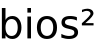
\includegraphics[scale=0.4]{fig/logo-bios2}\hfill
  
\includegraphics[scale=0.25]{fig/logo-csbq.png}\hfill
  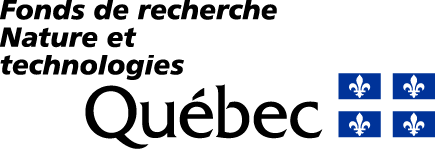
\includegraphics[scale=0.5]{fig/logo-frqnt.png}
}

\begin{document}

\begin{frame}
  \titlepage
\end{frame}

\begin{frame}
  \frametitle{Objective}
  Bring together 2 elements:
  \vfill
  \begin{enumerate}
    \item Identification of beta diversity hotspots $\rightarrow$ LCBD calculation
    \item Species distribution modelling on continuous scales $\rightarrow$ SDMs
  \end{enumerate}
  \vfill
  \begin{figure}
    \centering
    \hspace*{0.0cm}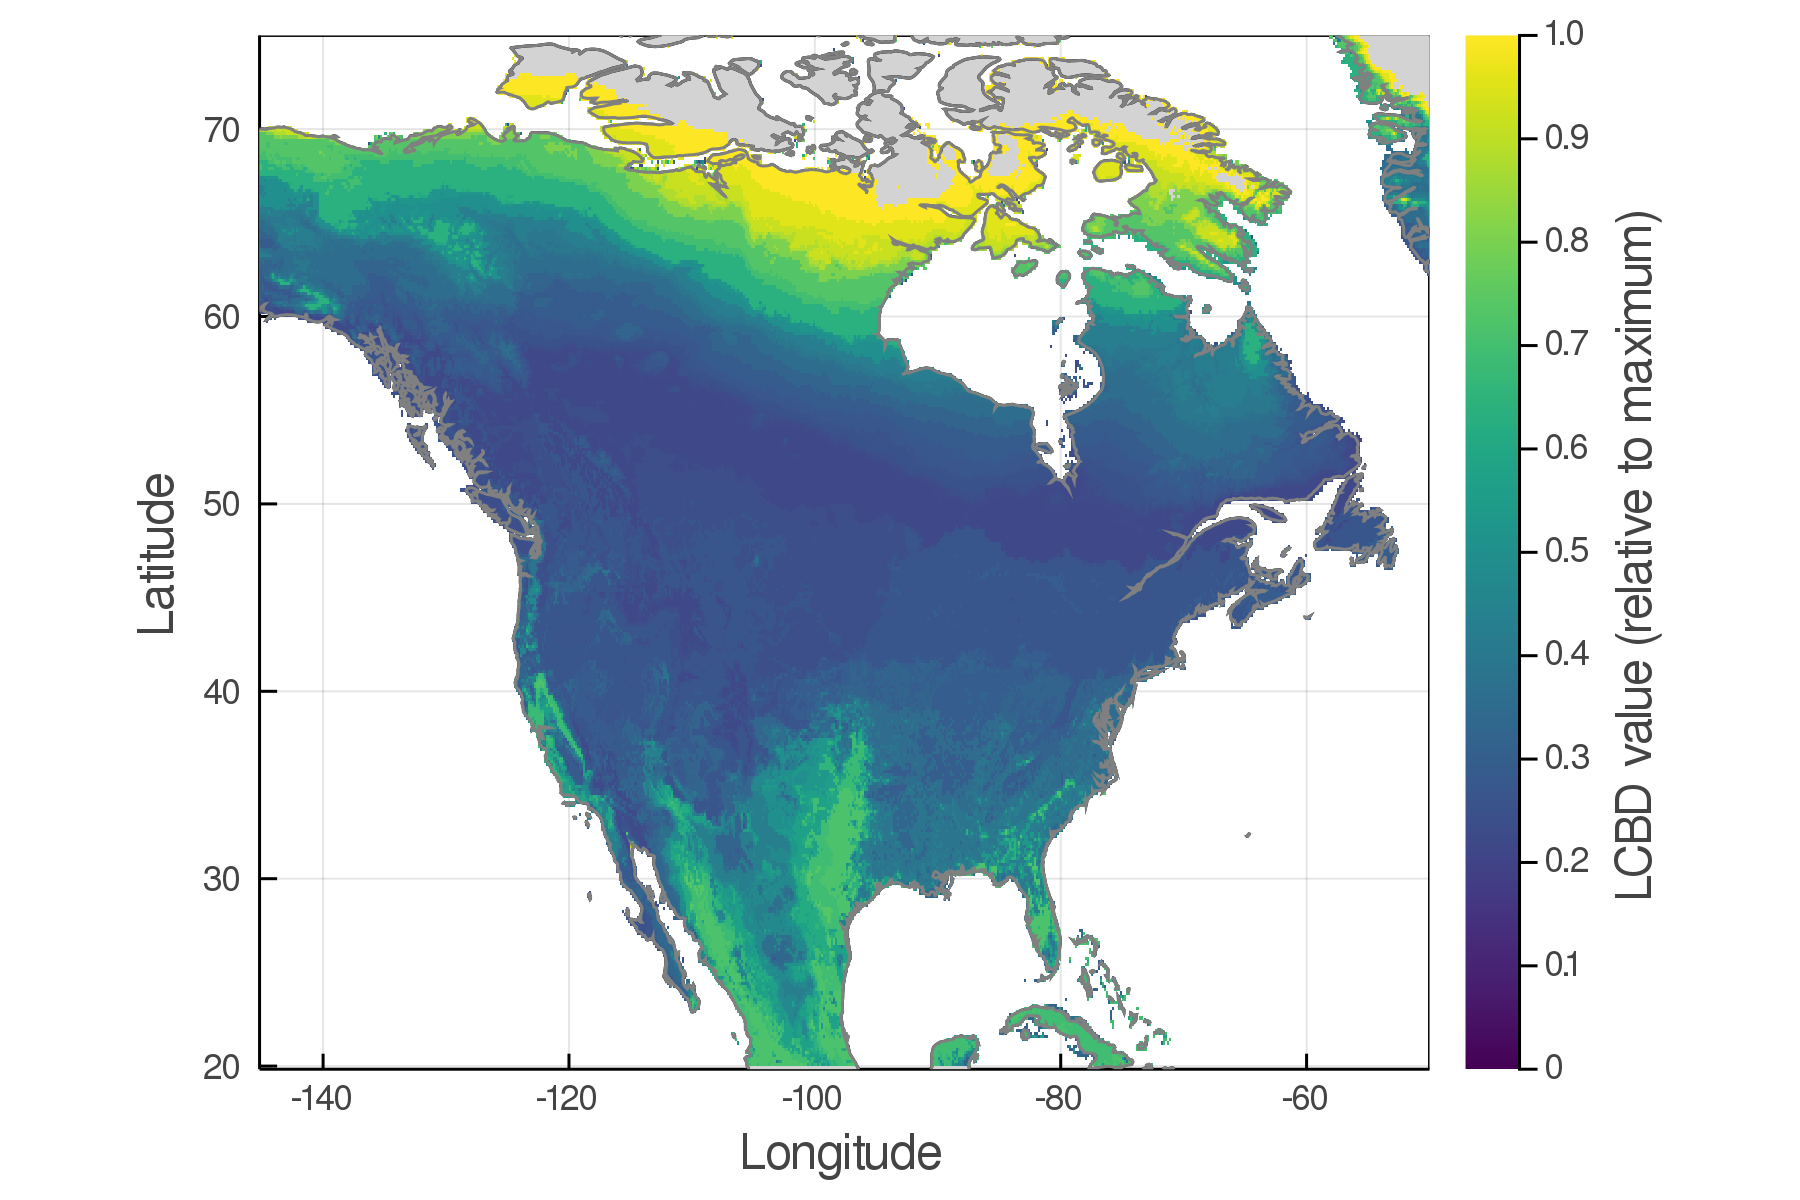
\includegraphics[scale=0.12]{fig/05_sdm_lcbd.png}
  \end{figure}
\end{frame}

\begin{frame}
  \frametitle{Why continuous scales?}
  \begin{figure}
    \centering
    \hspace*{-0cm}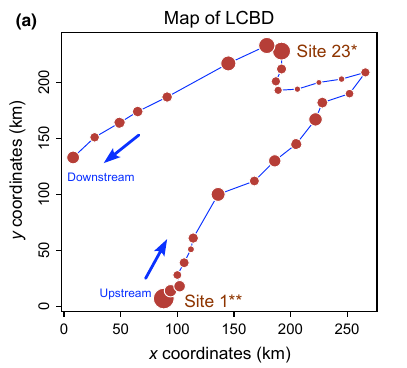
\includegraphics[scale=0.5]{fig/lcbd_LegeDeCa2013.png}
    \caption{Example of discontinuous LCBD calculation along a river stream (Legendre \& De Caceres, 2013)}
  \end{figure}
\end{frame}

\begin{frame}
  \frametitle{Why continuous scales?}
  \begin{figure}
    \centering
    \hspace*{-0cm}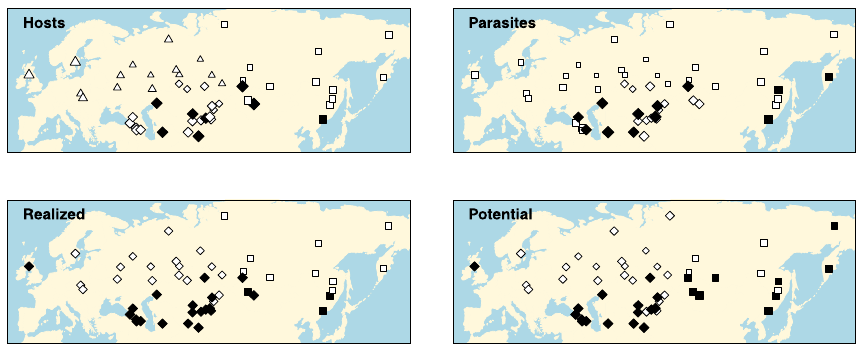
\includegraphics[scale=0.35]{fig/lcbd_Pois2017.png}
    \caption{Example of discontinuous LCBD calculation on an extended scale (Poisot et al., 2017)}
  \end{figure}
\end{frame}

\begin{frame}
  \frametitle{Why continuous scales?}
  \begin{itemize}
    \item Online data on extended scales is increasingly accessible
    \item Potential for novel ecological insights
  \end{itemize}
  \begin{figure}
    \centering
    \hspace*{-1cm}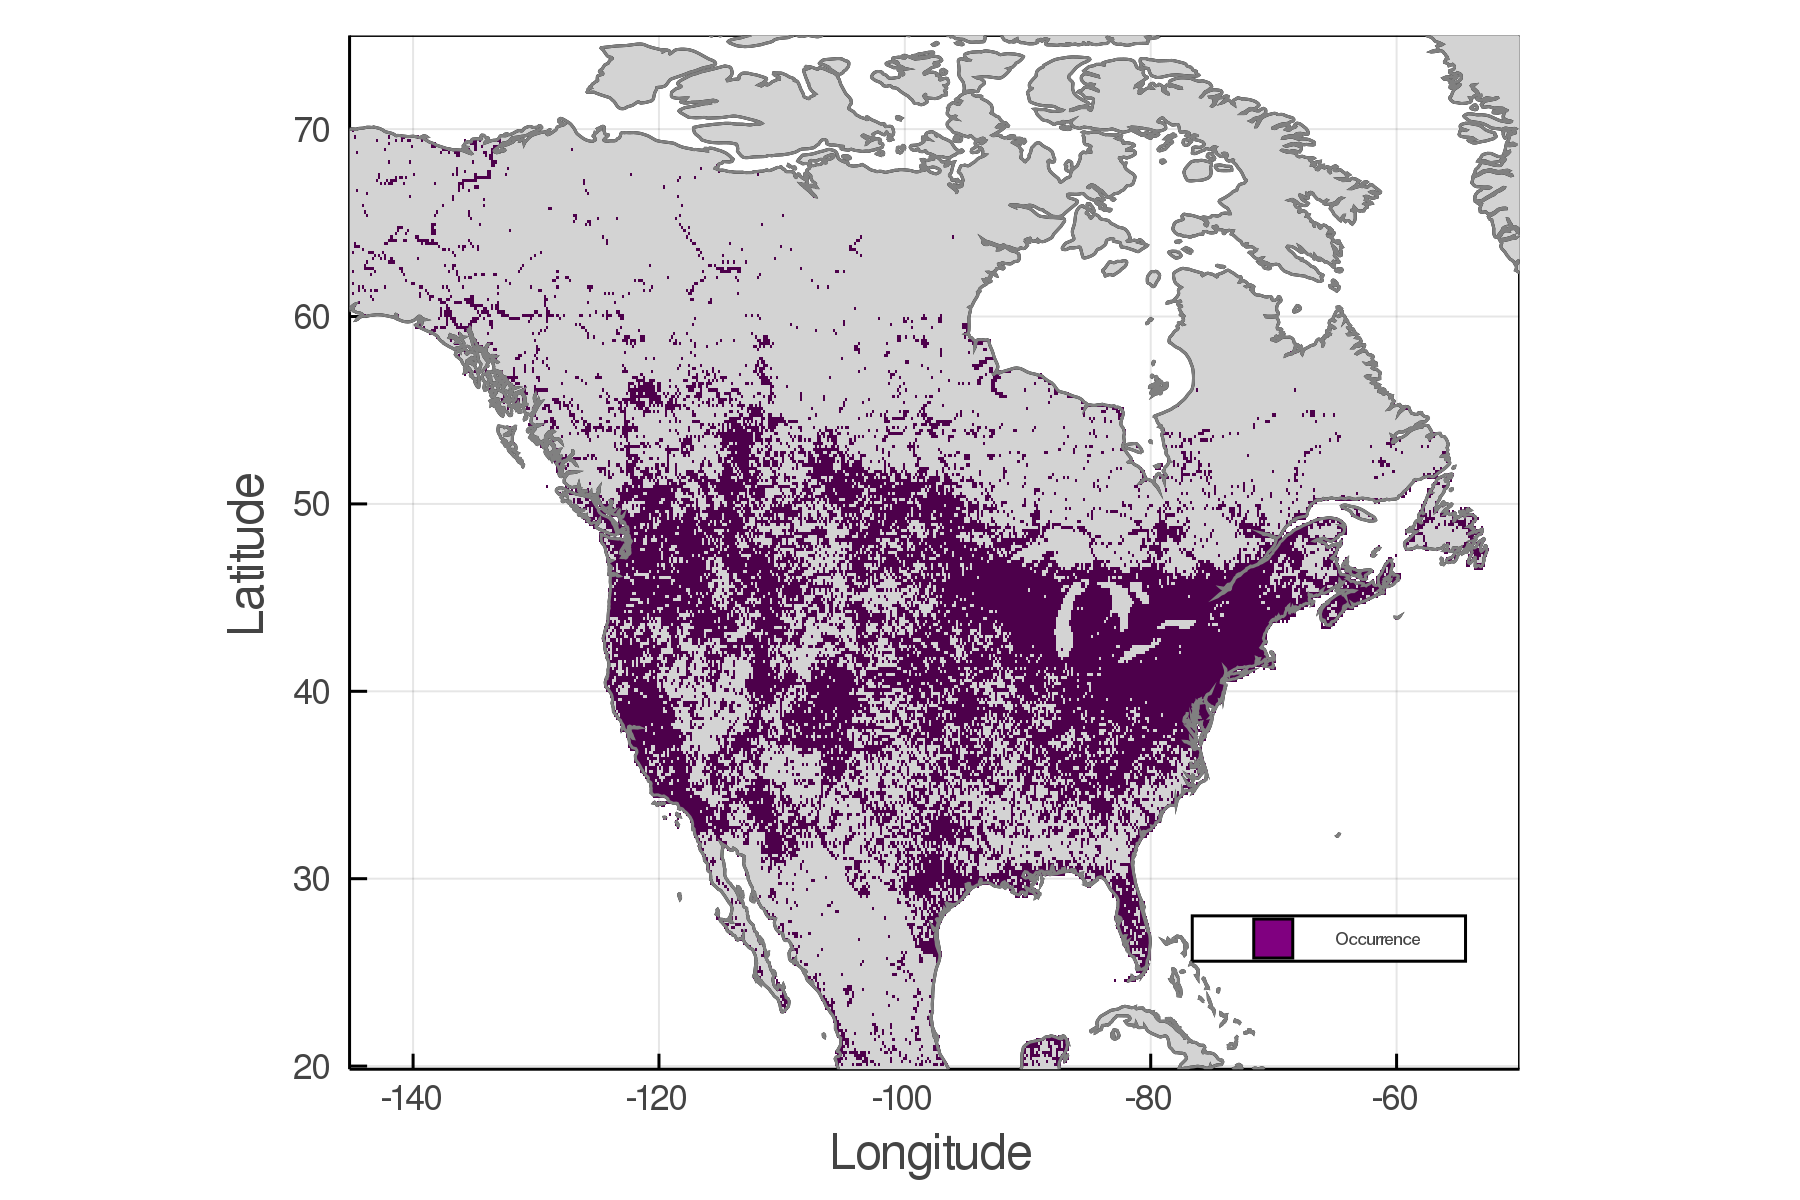
\includegraphics[scale=0.10]{fig/01_raw_singlesp.png}%
    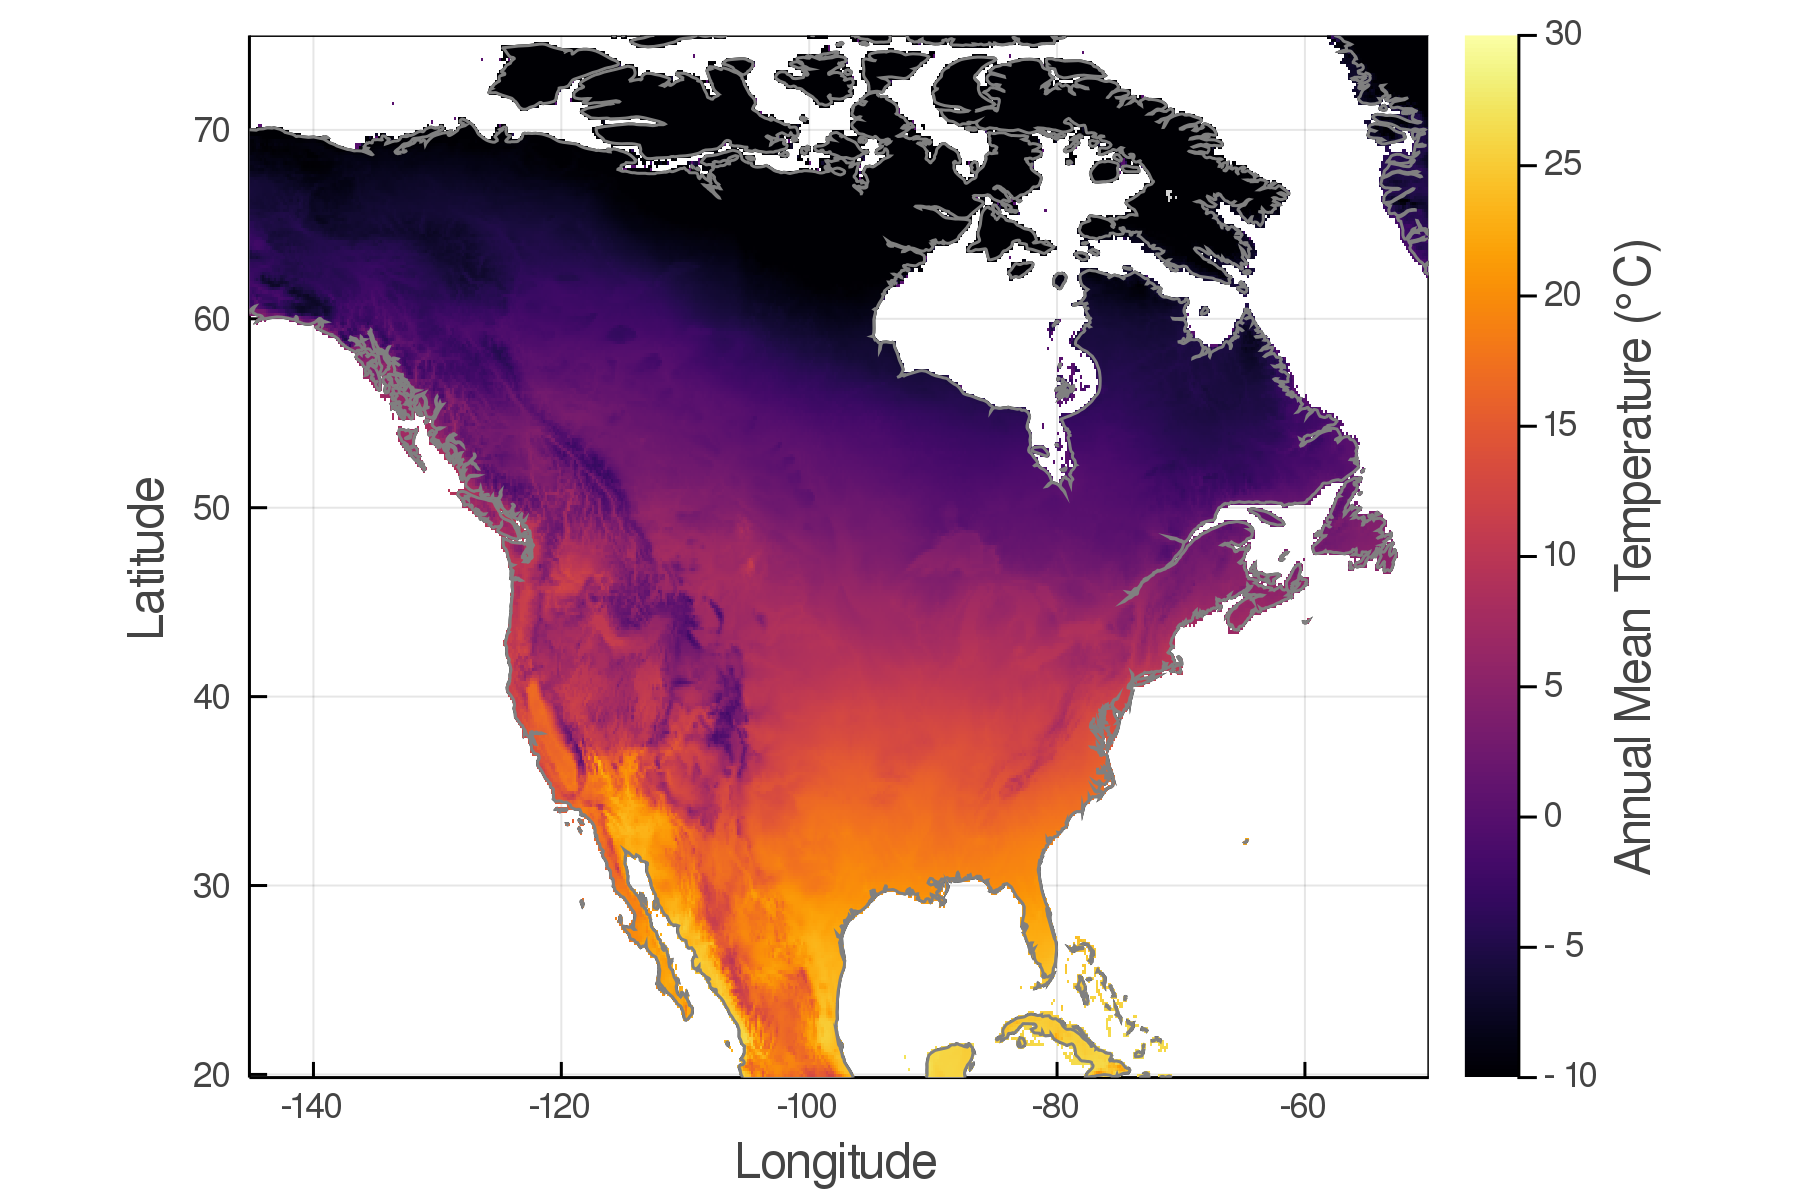
\includegraphics[scale=0.10]{fig/wc_temp.png}
    \caption{Example of Yellow Warbler occurrence data from eBird (left) and  annual mean temperature data from WorldClim 2 (right)}
  \end{figure}
\end{frame}

\begin{frame}
  \frametitle{Objective}
  \begin{figure}
    \centering
    \hspace*{-0cm}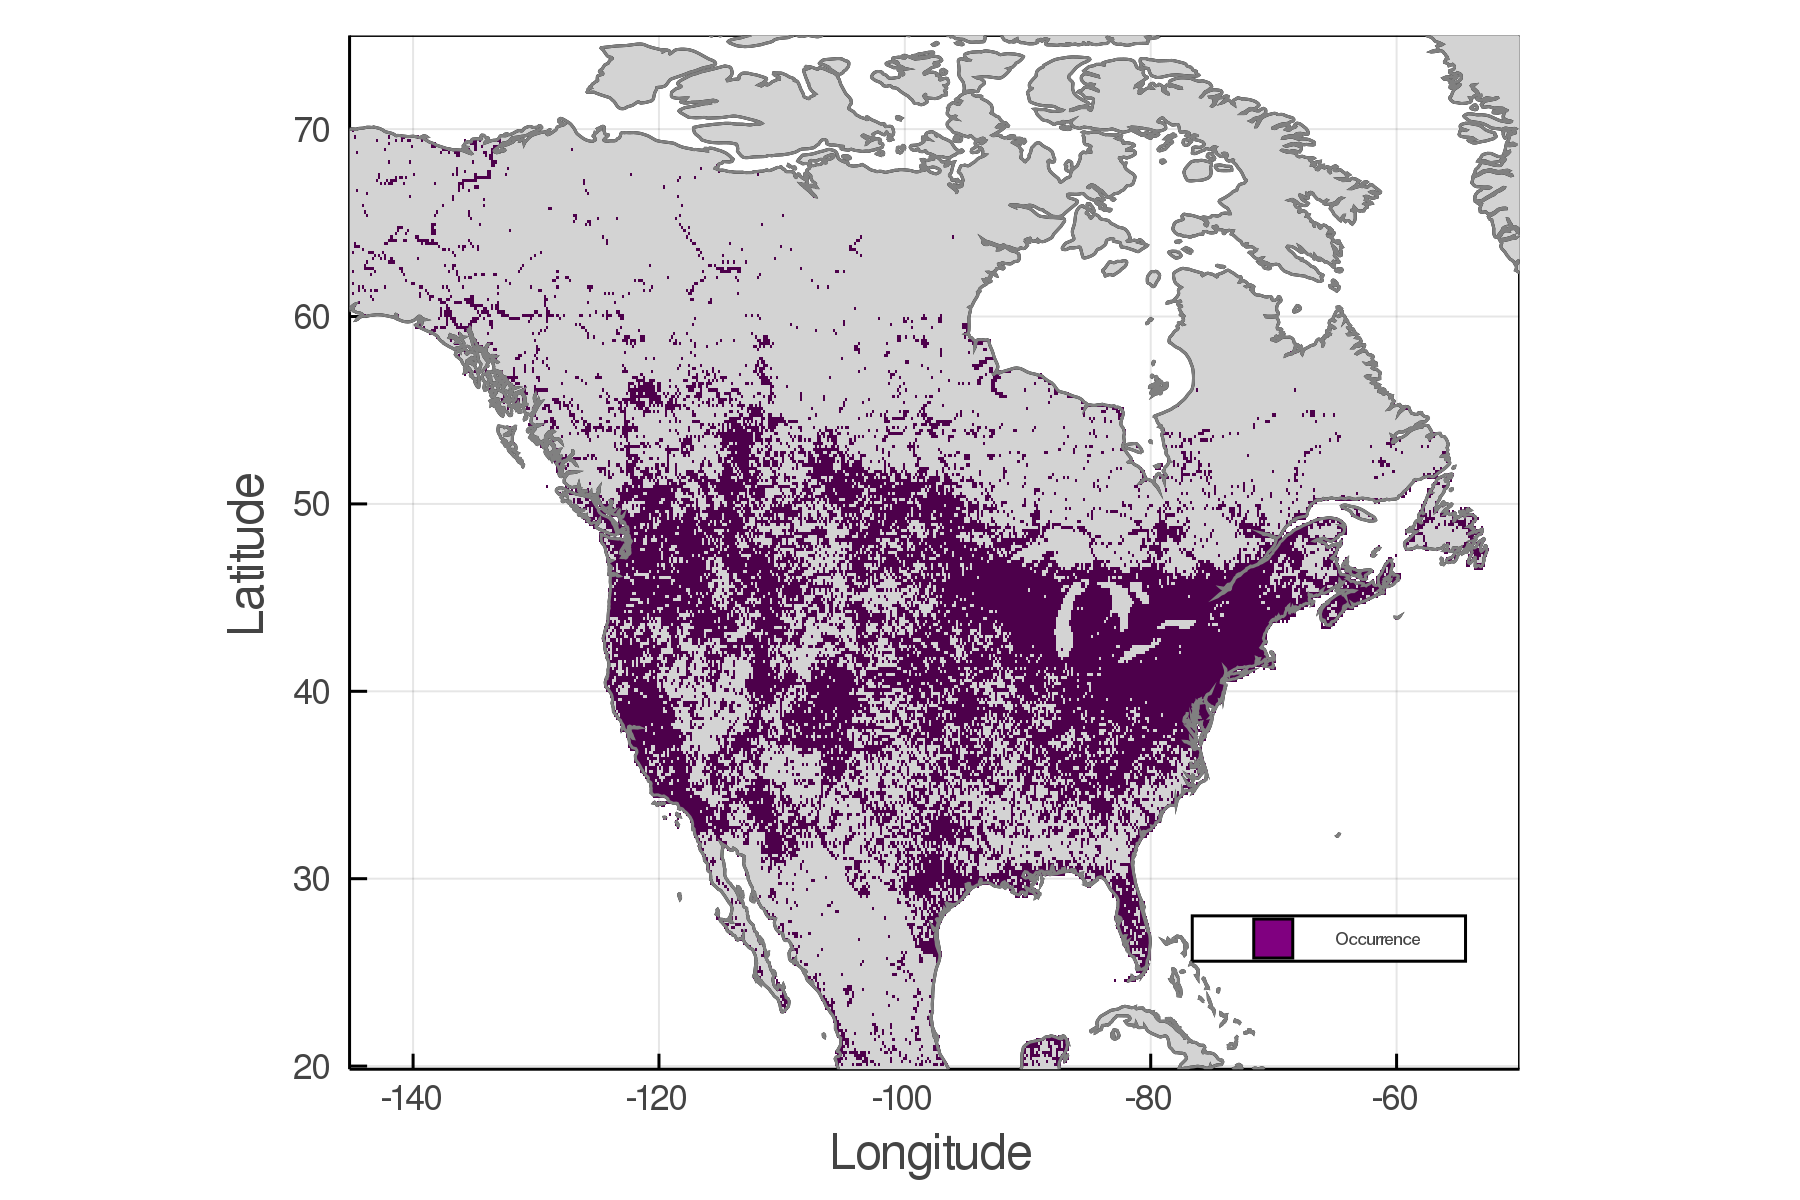
\includegraphics[scale=0.06]{fig/01_raw_singlesp.png}%
    \hspace*{0cm}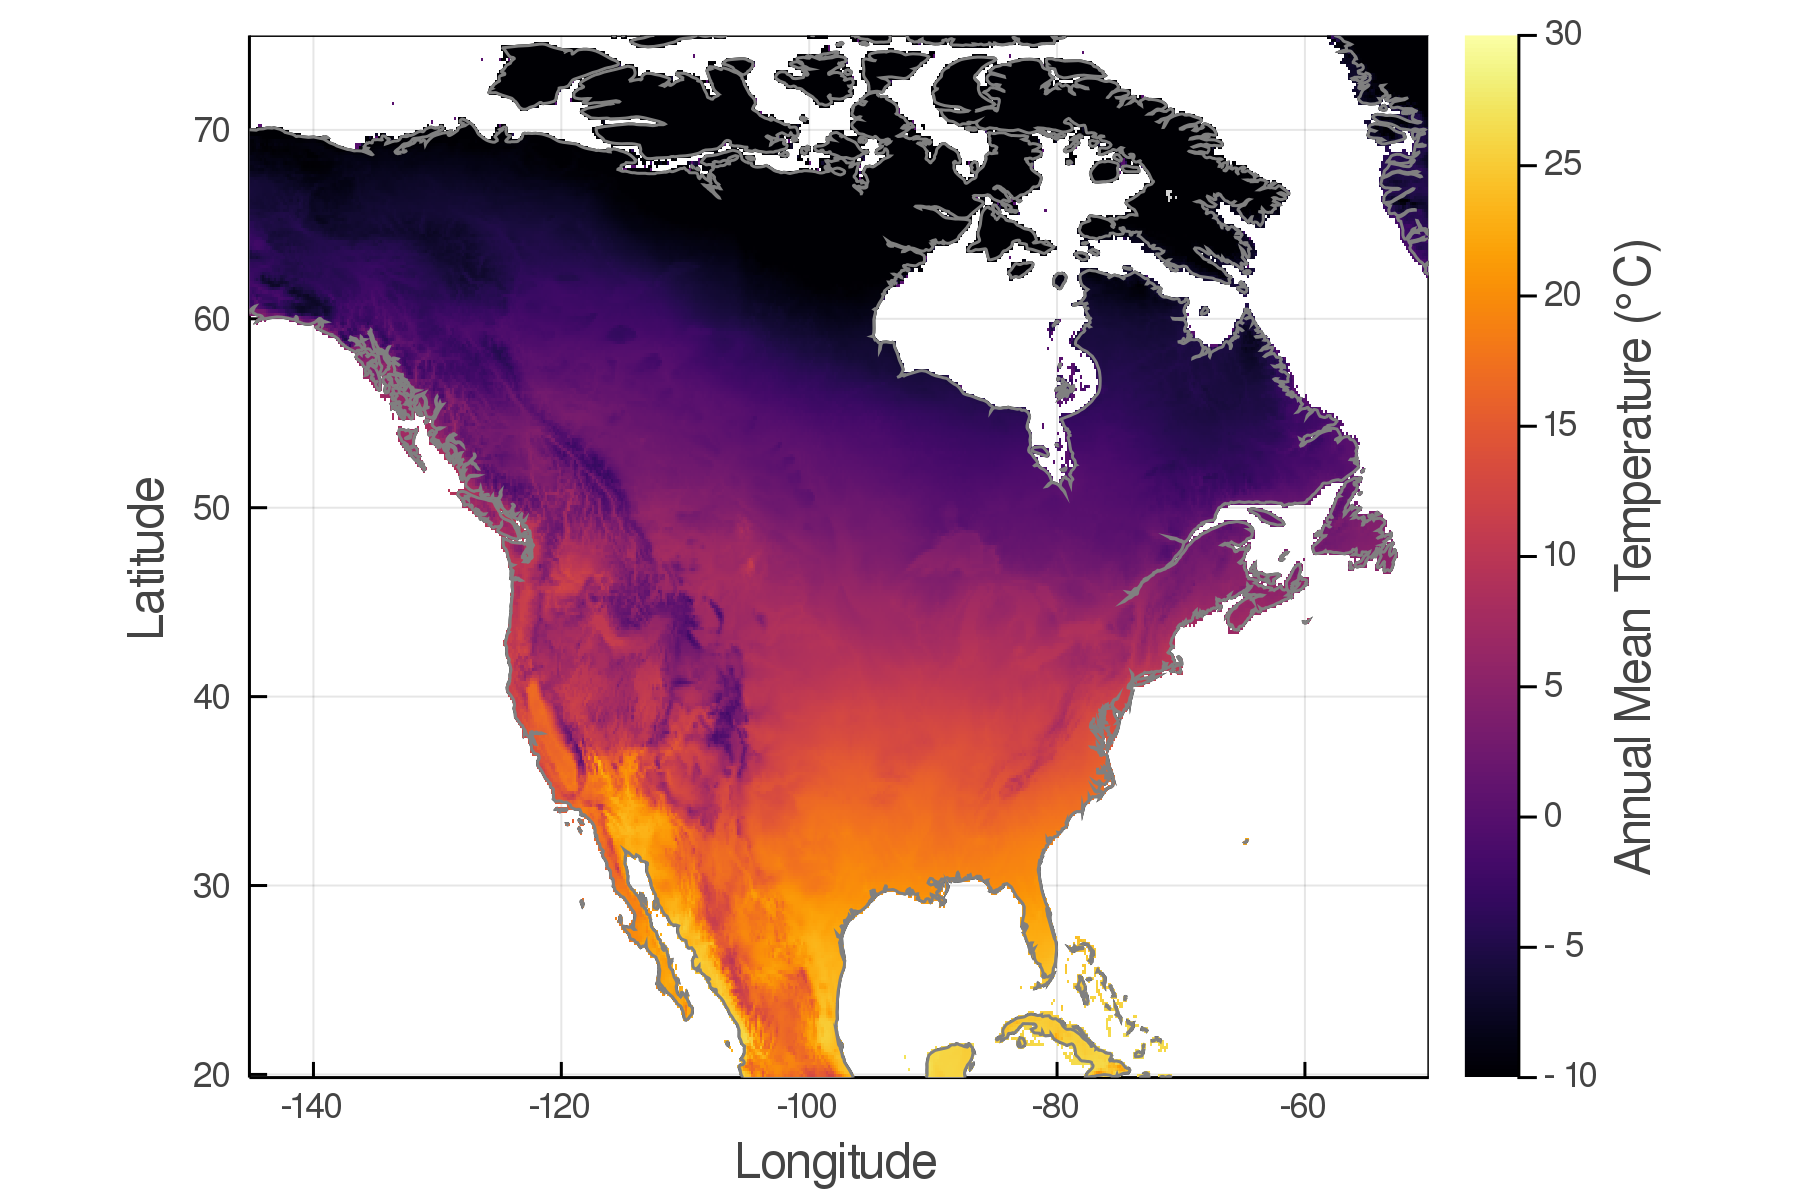
\includegraphics[scale=0.06]{fig/wc_temp.png}
    \vfill
    $\Downarrow$
    \vfill
    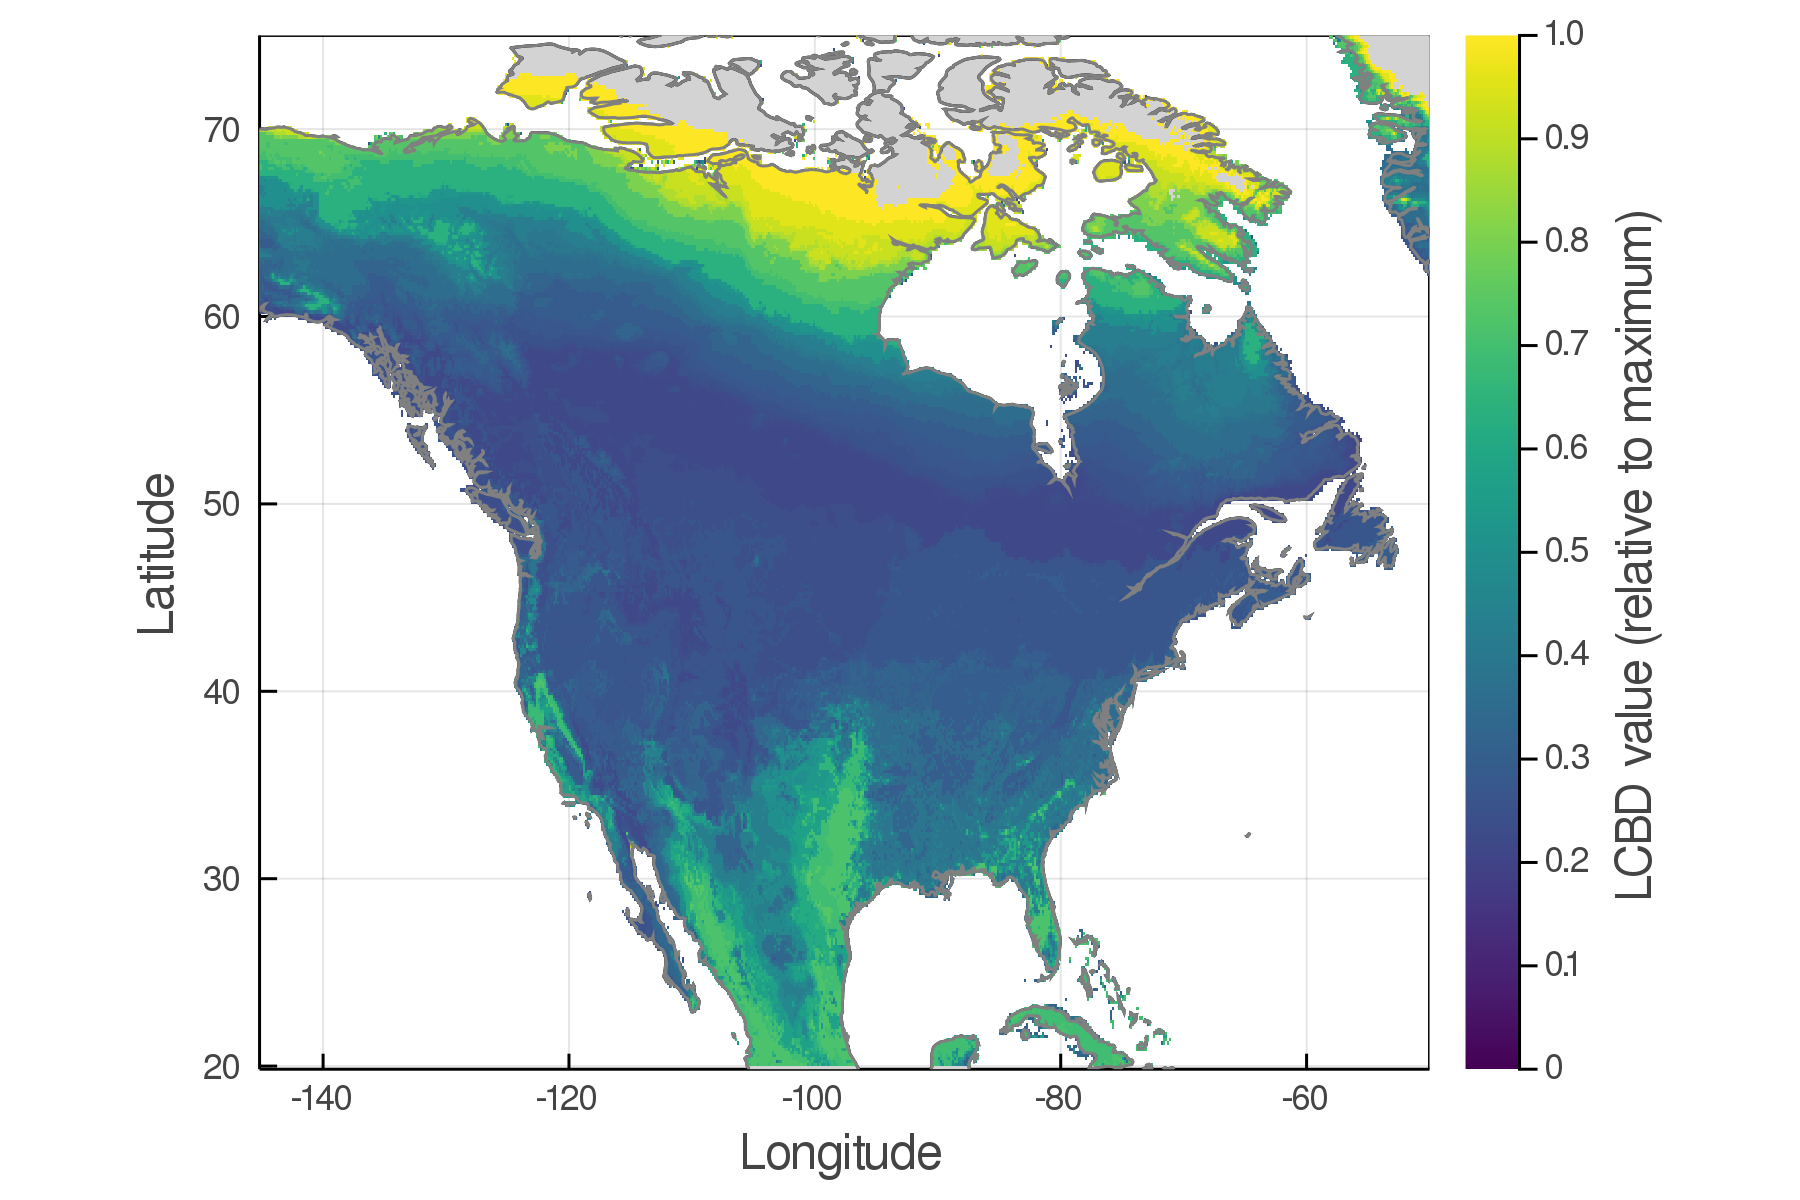
\includegraphics[scale=0.10]{fig/05_sdm_lcbd.png}
  \end{figure}
\end{frame}

\begin{frame}
  \frametitle{Relevance}
  \begin{columns}
    \hspace*{-0cm}\column{0.6\textwidth}
      Novel ecological insights
      \begin{itemize}
        \item Tool for poorly sampled regions, or with sparse sampling
        \item Identification of conservation targets
      \end{itemize}
      \vspace{0.5cm}
      Combination with IPCC climate change scenarios
      \begin{itemize}
        \item Model beta diversity changes
        \item Identify sites with significant changes
      \end{itemize}
      \vspace{0.5cm}
    \hspace*{-1cm}\column{0.5\textwidth}
      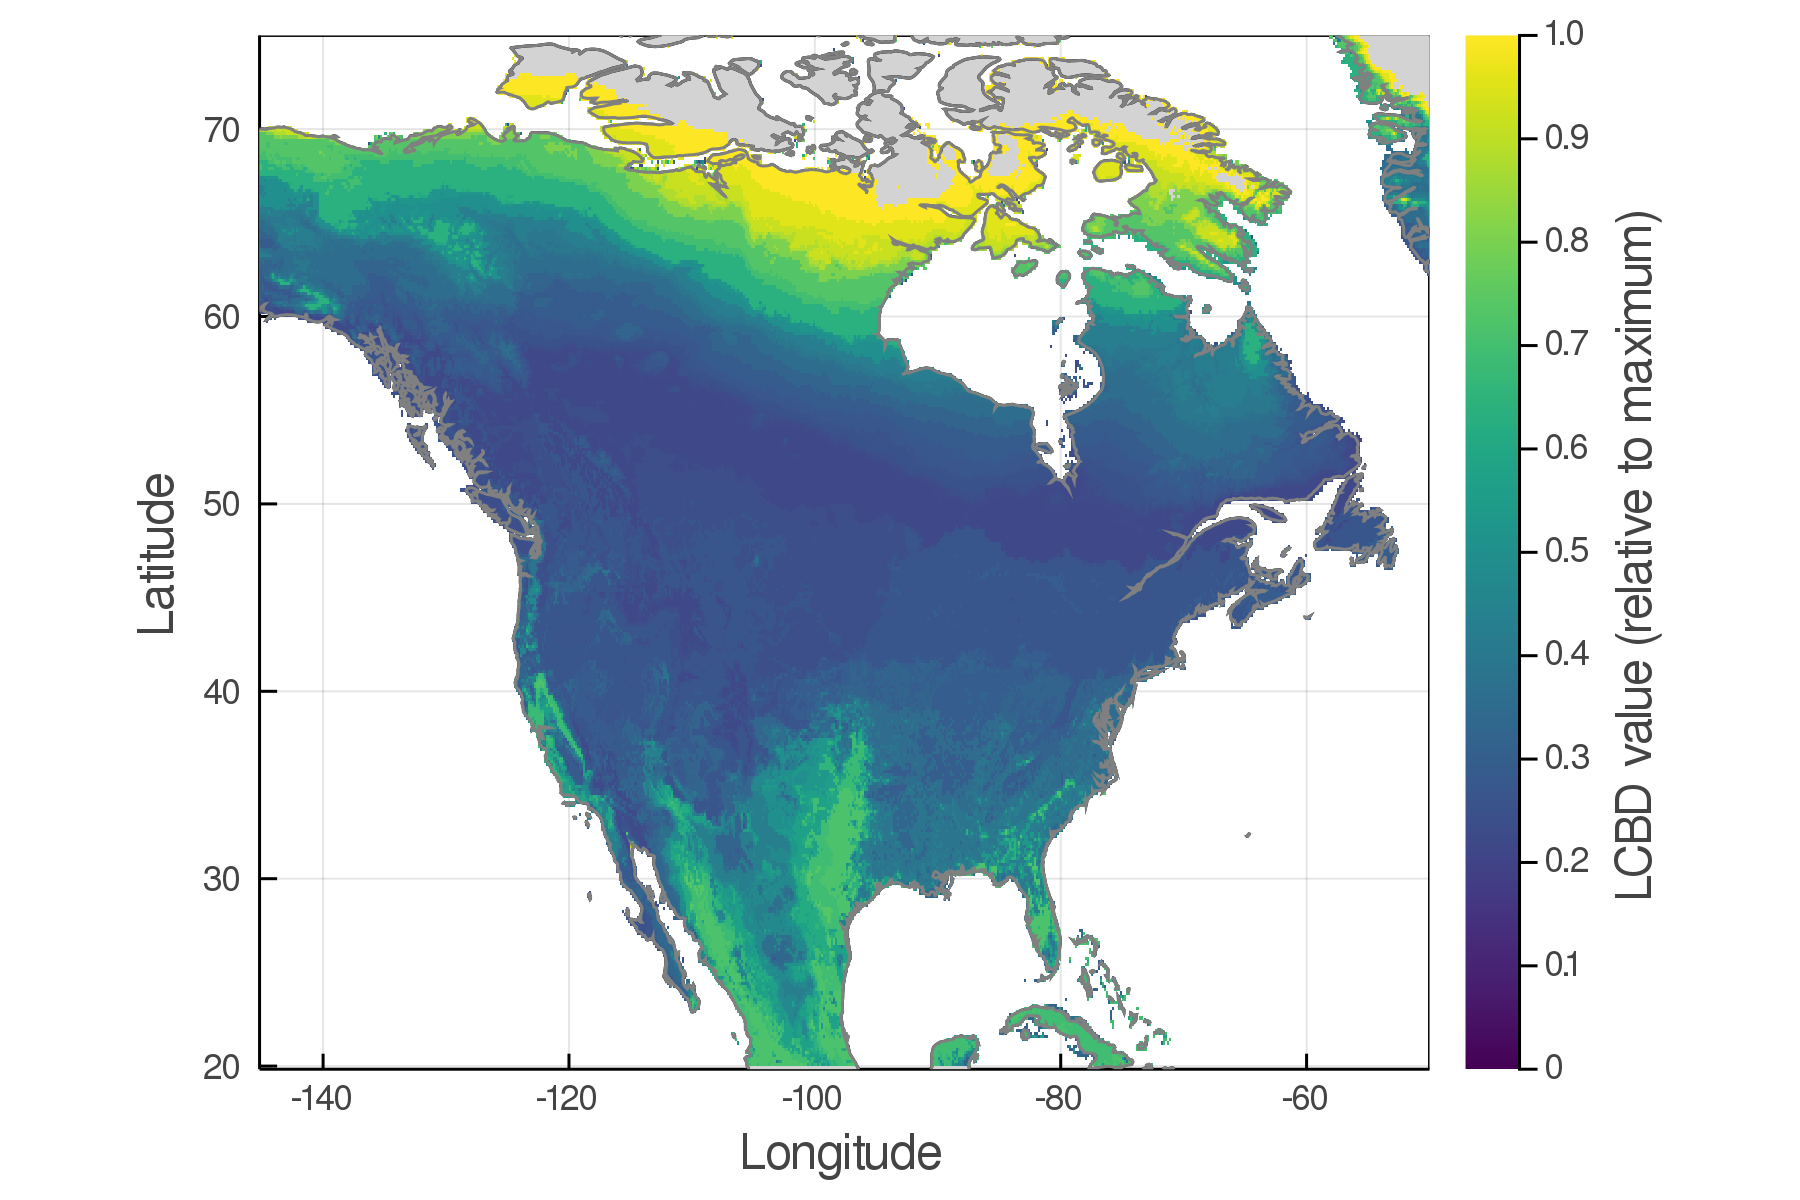
\includegraphics[scale=0.10]{fig/05_sdm_lcbd.png}
  \end{columns}
  $\Rightarrow$ Insight-oriented approach, exploratory analyses for now
\end{frame}

\begin{frame}
  \frametitle{Data - Why eBird \& Warblers}
  According to Johnston et al. (2019):
  \begin{enumerate}
    \item Complete checklists to infer absences
    \item Sampling effort metadata to reduce biases
  \end{enumerate}
  % Use adjustbox to display despite large width
  % Caption as to be in adjust box, not table
  \begin{adjustbox}{center, caption={Structure of the Warblers (\textit{Parulidae}) occurrence data for North America in the eBird complete checklists}, float=table}
    \begin{table}
      \scriptsize
      % Reset table row width, doesn't follow default for some reason
      \def\arraystretch{1.5}
      \hspace{}\begin{tabularx}{1.1\textwidth}{X X X X X X X}
      \hline
      Country & Observations & Checklists & Species & Species per checklist (mean) & Species per checklist (median) & Species per checklist (max) \\
      \hline
      US    & 19 206 453 & 7 840 526 & 56 & 2.450 & 2.0 & 34 \\
      CA    & 3 360 650  & 1 115 625 & 45 & 3.012 & 2.0 & 31 \\
      MX    & 407 227    & 147 599   & 61 & 2.759 & 2.0 & 21 \\
      Total & 22 974 330 & 9 103 750 & 63 & 2.523 & 2.0 & 34 \\
      \hline
    \end{tabularx}
  \end{table}
 \end{adjustbox}
\end{frame}

\begin{frame}
  \frametitle{Data - Why WorldClim 2 }
  \begin{columns}
    \begin{column}{0.5\textwidth}
      \begin{itemize}
        \item Interpolated climate data
        \item Global range
        \item Resolutions from 10 arc-minutes to 30 arc-seconds
        \item 2 types of variables: temperature, precipitation
        \item High cross-validation coefficients
      \end{itemize}
    \end{column}
    \begin{column}{0.5\textwidth}
      \centering
      \resizebox{1.0\textwidth}{!}{%
      \begin{table}
        \small
        %\caption{test}
        \begin{tabular}{c l}
          \hline
          Variable & Description                            \\
          \hline
          1        & Annual Mean Temperature                \\
          2        & Mean Diurnal Range                     \\
          3        & Isothermality                          \\
          4        & Temperature Seasonality                \\
          5        & Max Temperature of Warmest Month       \\
          6        & Min Temperature of Coldest Month       \\
          7        & Temperature Annual Range               \\
          8        & Mean Temperature of Wettest Quarter    \\
          9        & Mean Temperature of Driest Quarter     \\
          10       & Mean Temperature of Warmest Quarter    \\
          11       & Mean Temperature of Coldest Quarter    \\
          \hline
          12       & Annual Precipitation                   \\
          13       & Precipitation of Wettest Month         \\
          14       & Precipitation of Driest Month          \\
          15       & Precipitation Seasonality              \\
          16       & Precipitation of Wettest Quarter       \\
          17       & Precipitation of Driest Quarter        \\
          18       & Precipitation of Warmest Quarter       \\
          19       & Precipitation of Coldest Quarter       \\
          \hline
        \end{tabular}
      \end{table}
    }
    \end{column}
  \end{columns}
\end{frame}

\begin{frame}
  \frametitle{Methods - BIOCLIM}
  \begin{figure}
    \centering
    \hspace*{-0cm}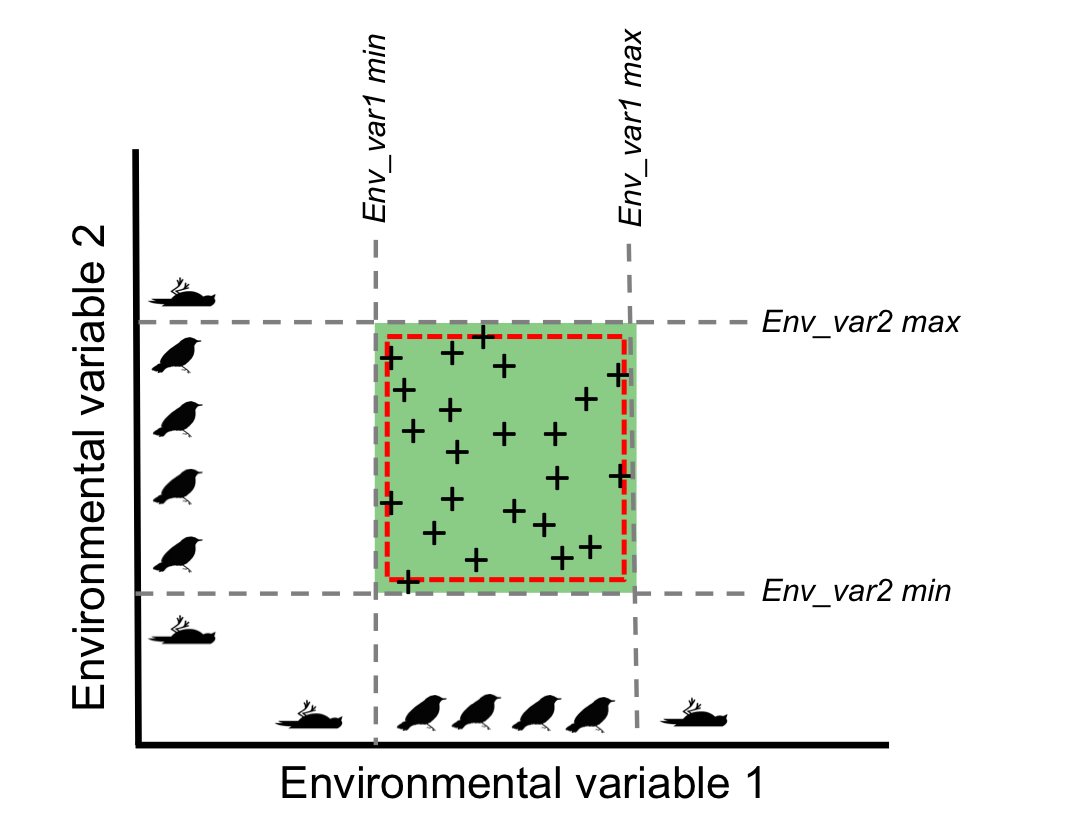
\includegraphics[scale=0.25]{fig/bioclim_bccvl.png}
    \caption{Representation of the climate envelope in the BIOCLIM method\footnote{\tiny https://support.bccvl.org.au/support/solutions/articles/6000083201-bioclim}}
  \end{figure}
\end{frame}

\begin{frame}
  \vfill
  \centering
  \huge Preliminary Results
  \vfill
\end{frame}

\begin{frame}
  \frametitle{Single species example - Raw data}
  \begin{figure}
    \centering
    \hspace*{-0cm}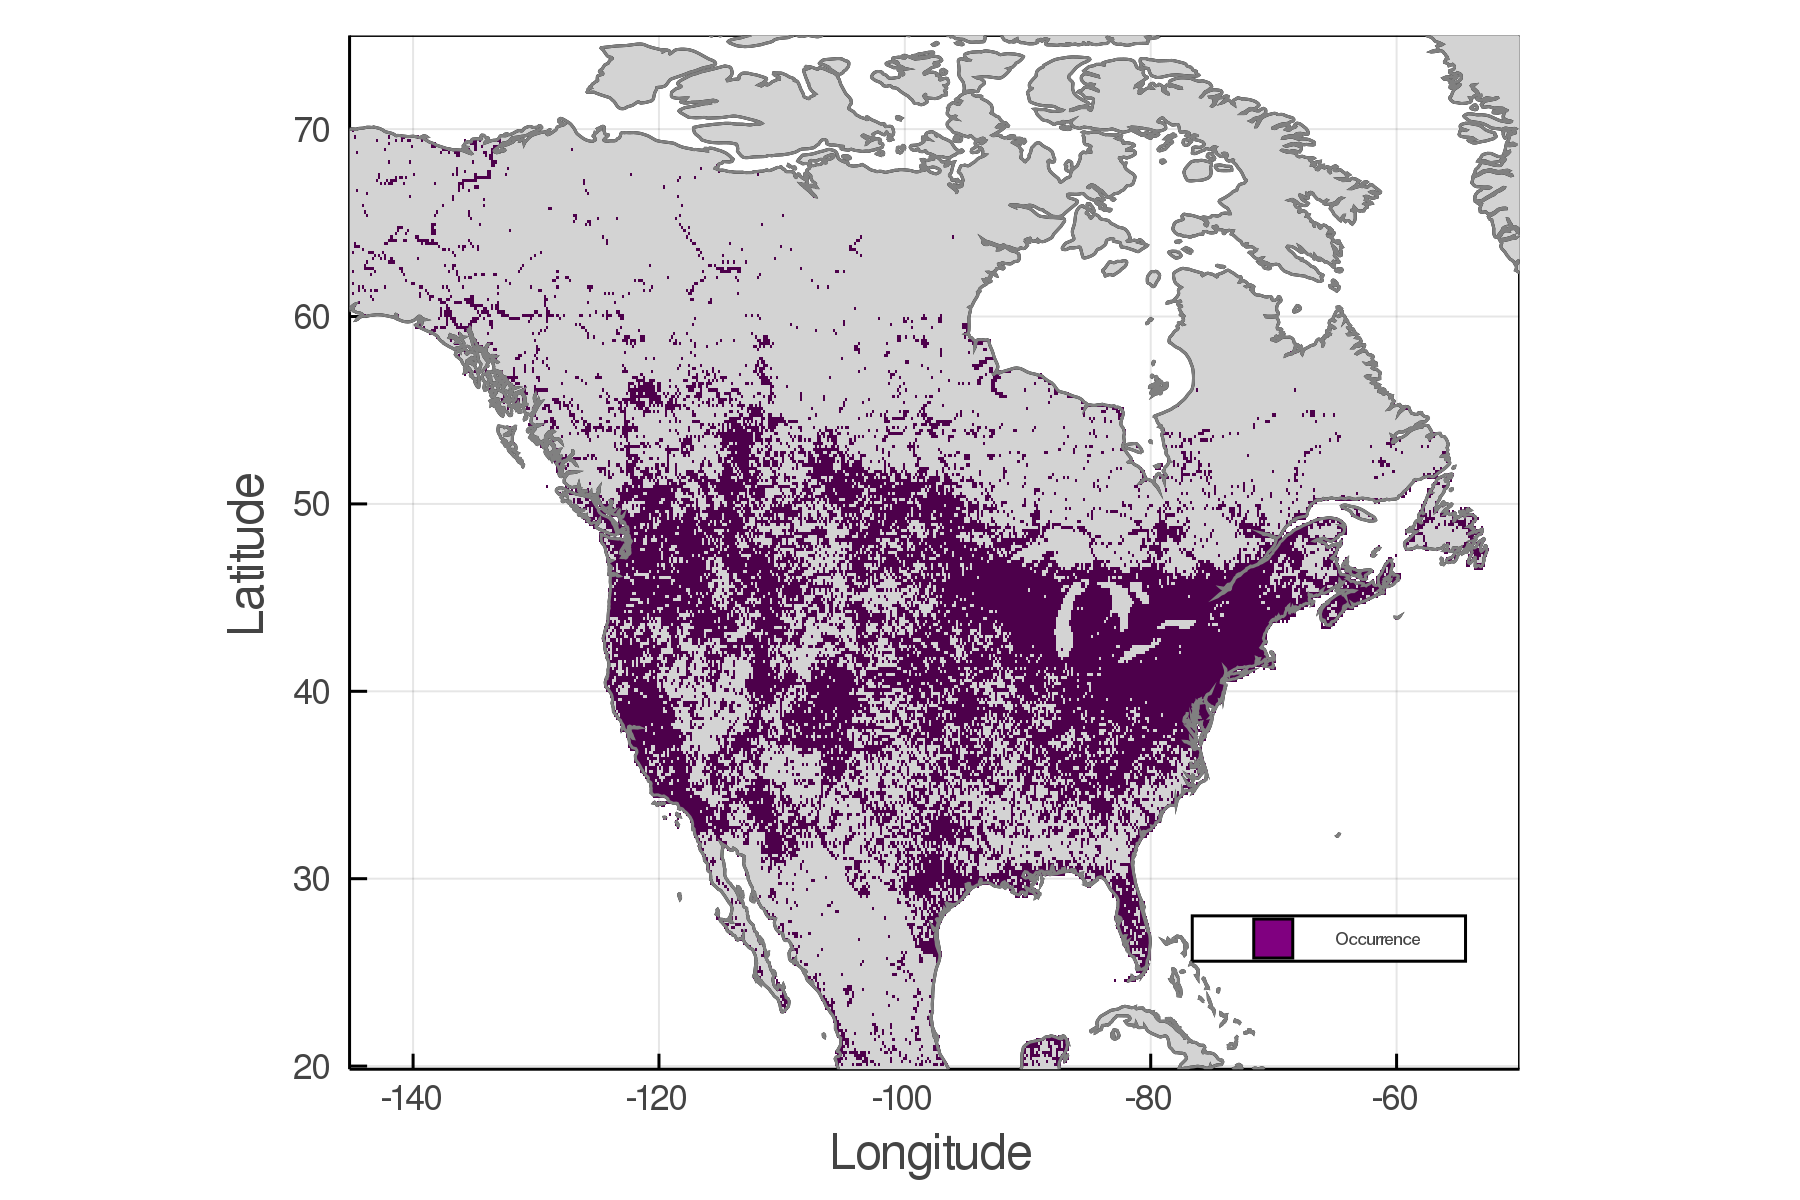
\includegraphics[scale=0.17]{fig/01_raw_singlesp.png}
    \caption{Distribution of the Yellow Warbler based on the raw occurrence data after transformation into presence-absence per site}
  \end{figure}
\end{frame}

\begin{frame}
  \frametitle{Single species example - SDM with threshold}
  \begin{figure}
    \centering
    \hspace*{-0cm}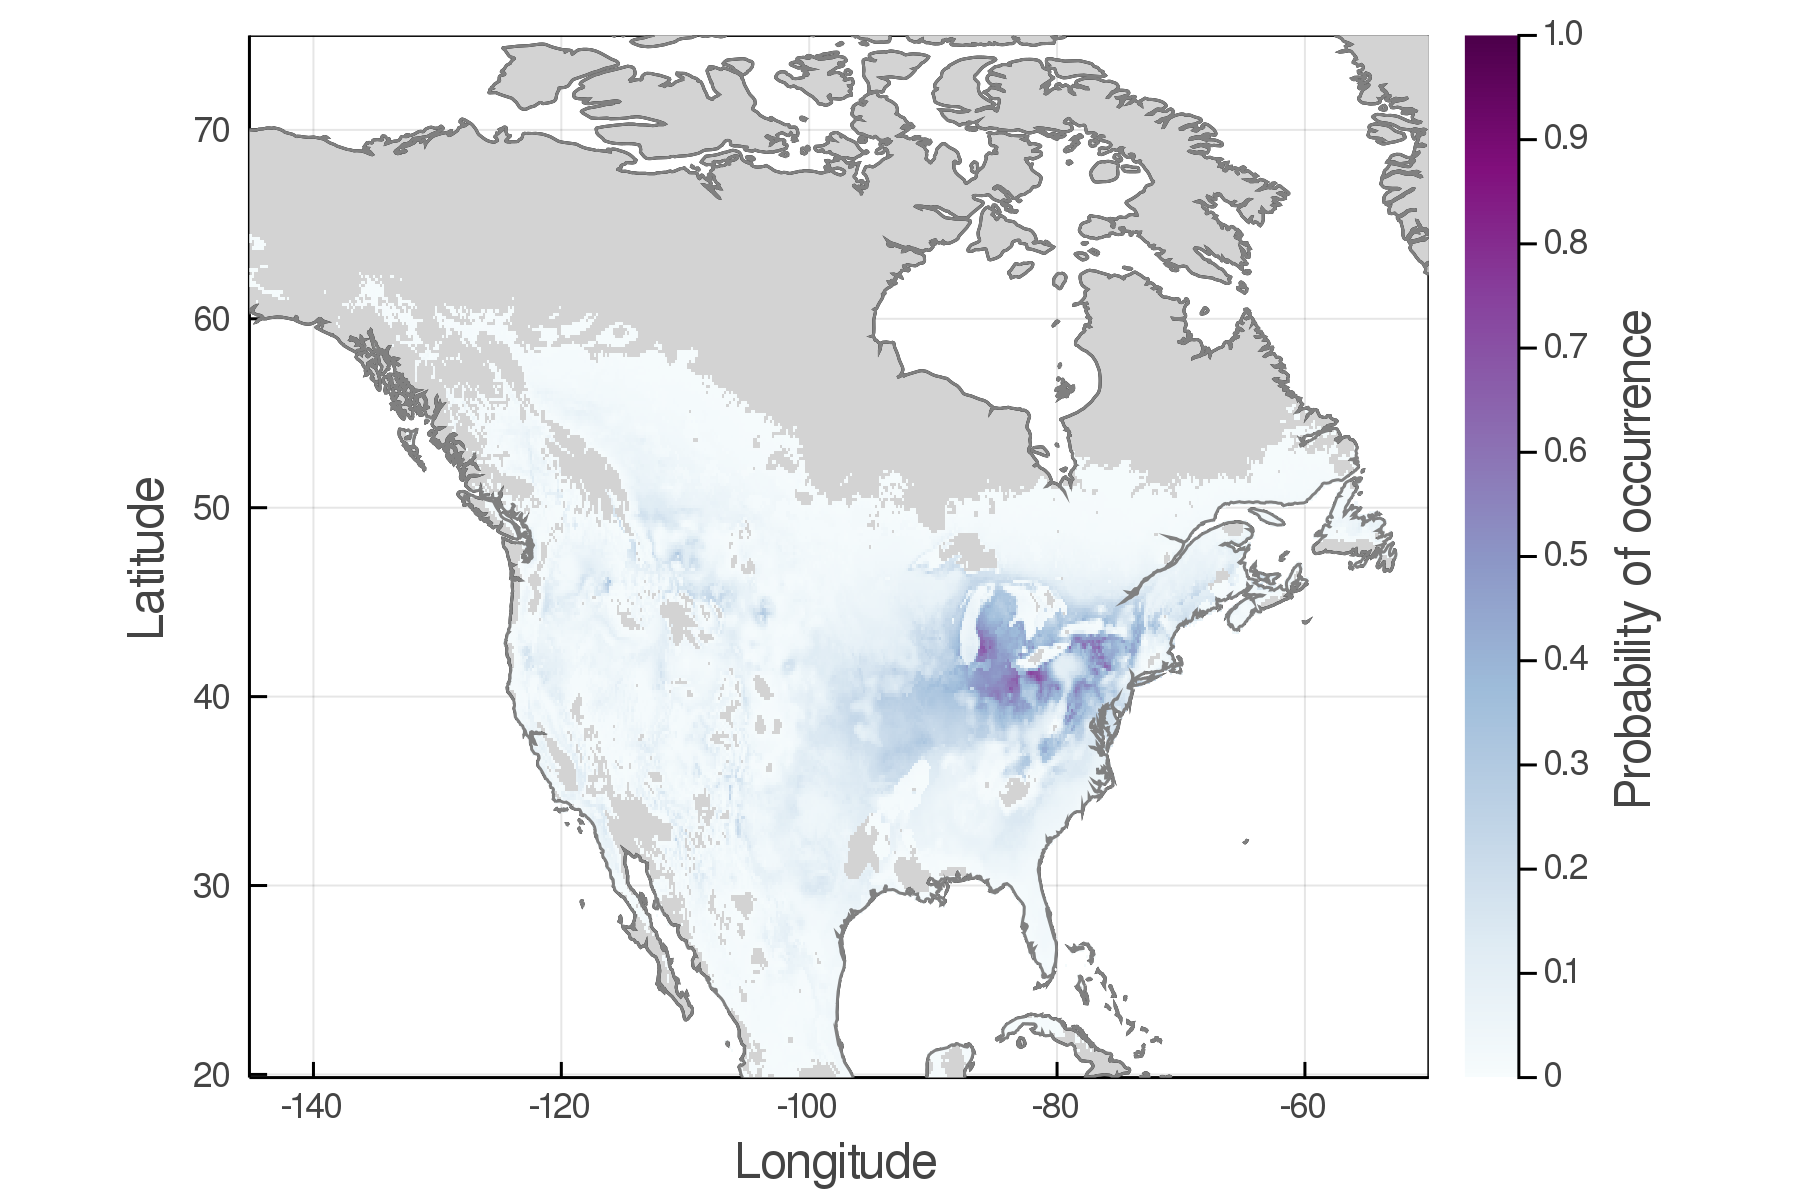
\includegraphics[scale=0.17]{fig/01_sdm_singlesp-threshold.png}
    \caption{Distribution of the Yellow Warbler based on the SDM predictions with a threshold of 5\%}
  \end{figure}
\end{frame}

\begin{frame}
  \frametitle{Single species example - SDM without threshold}
  \begin{figure}
    \centering
    \hspace*{-0cm}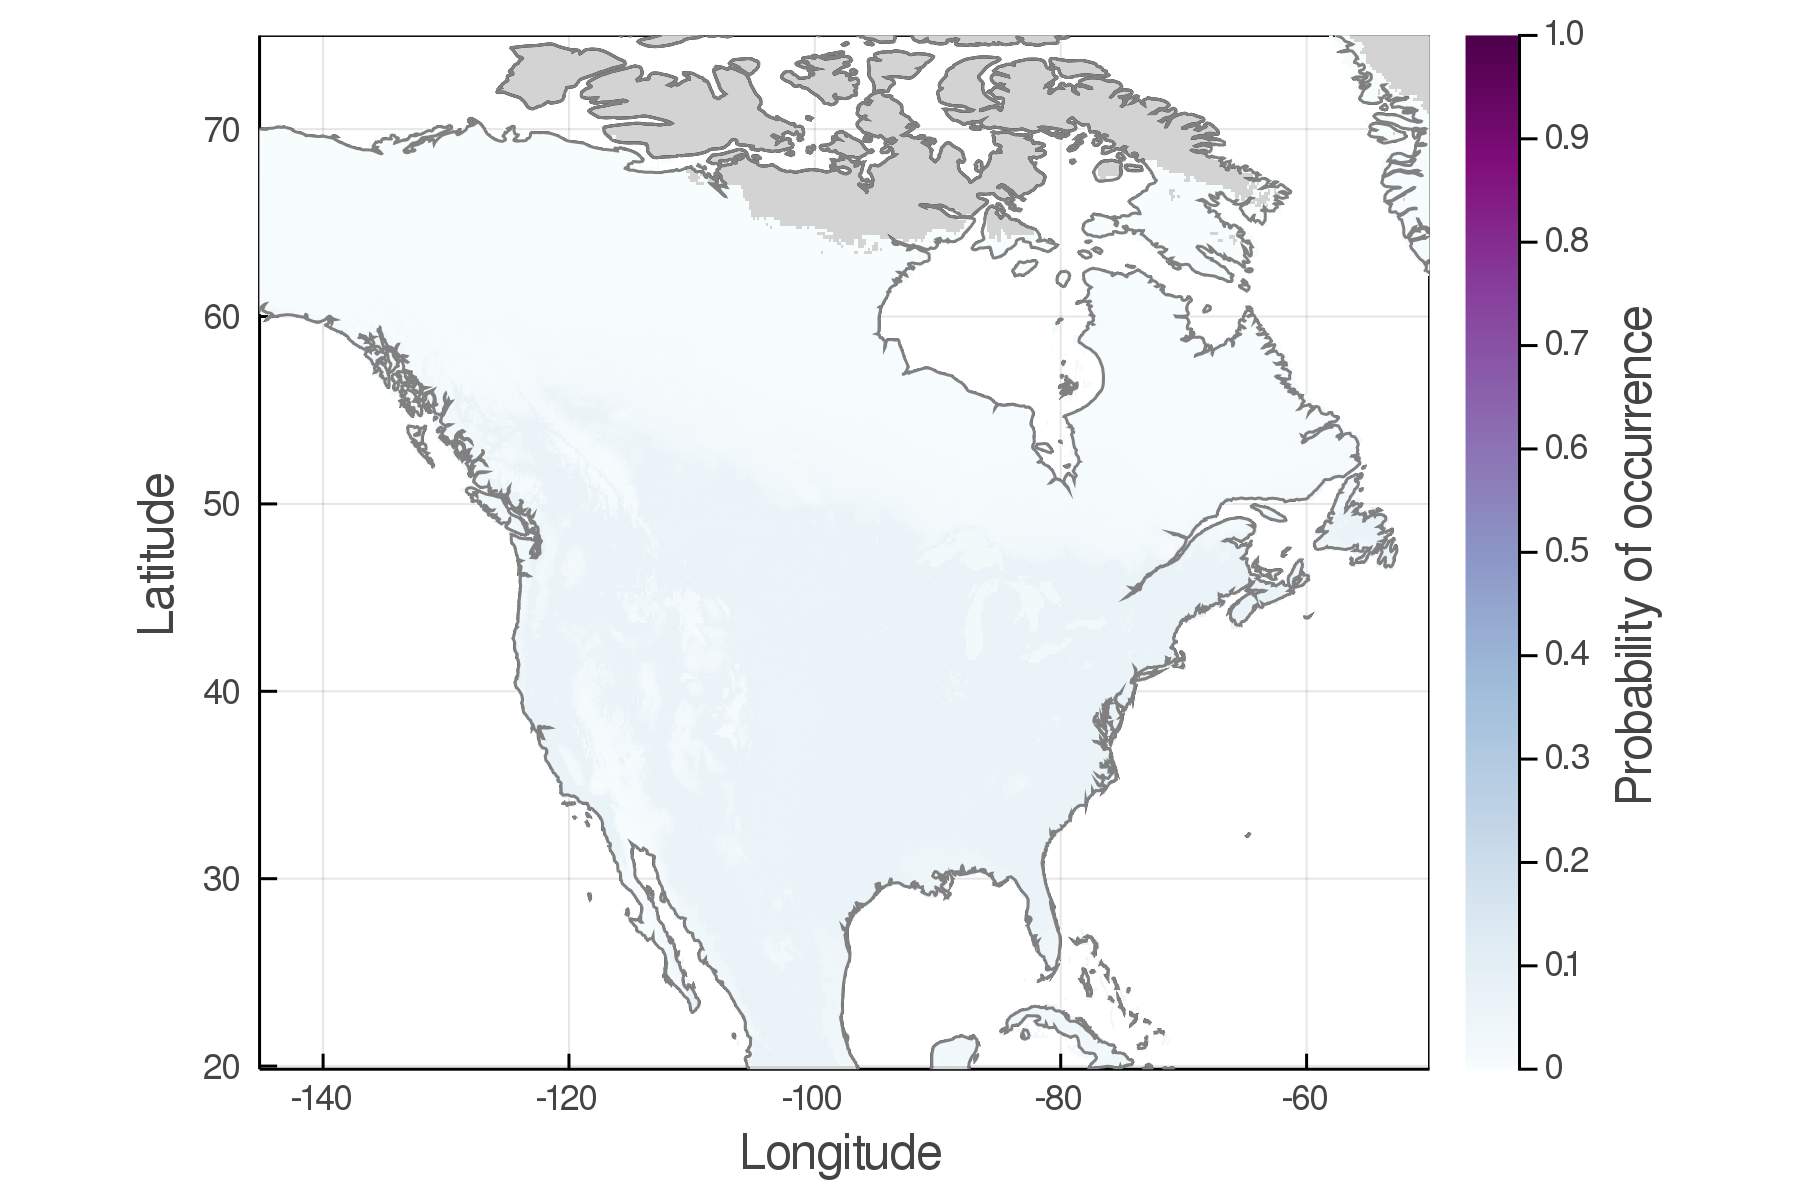
\includegraphics[scale=0.17]{fig/01_sdm_singlesp.png}
    \caption{Distribution of the Yellow Warbler based on the SDM predictions without a threshold}
  \end{figure}
\end{frame}

\begin{frame}
  \frametitle{Species richness - Raw data}
  \begin{figure}
    \centering
    \hspace*{-0cm}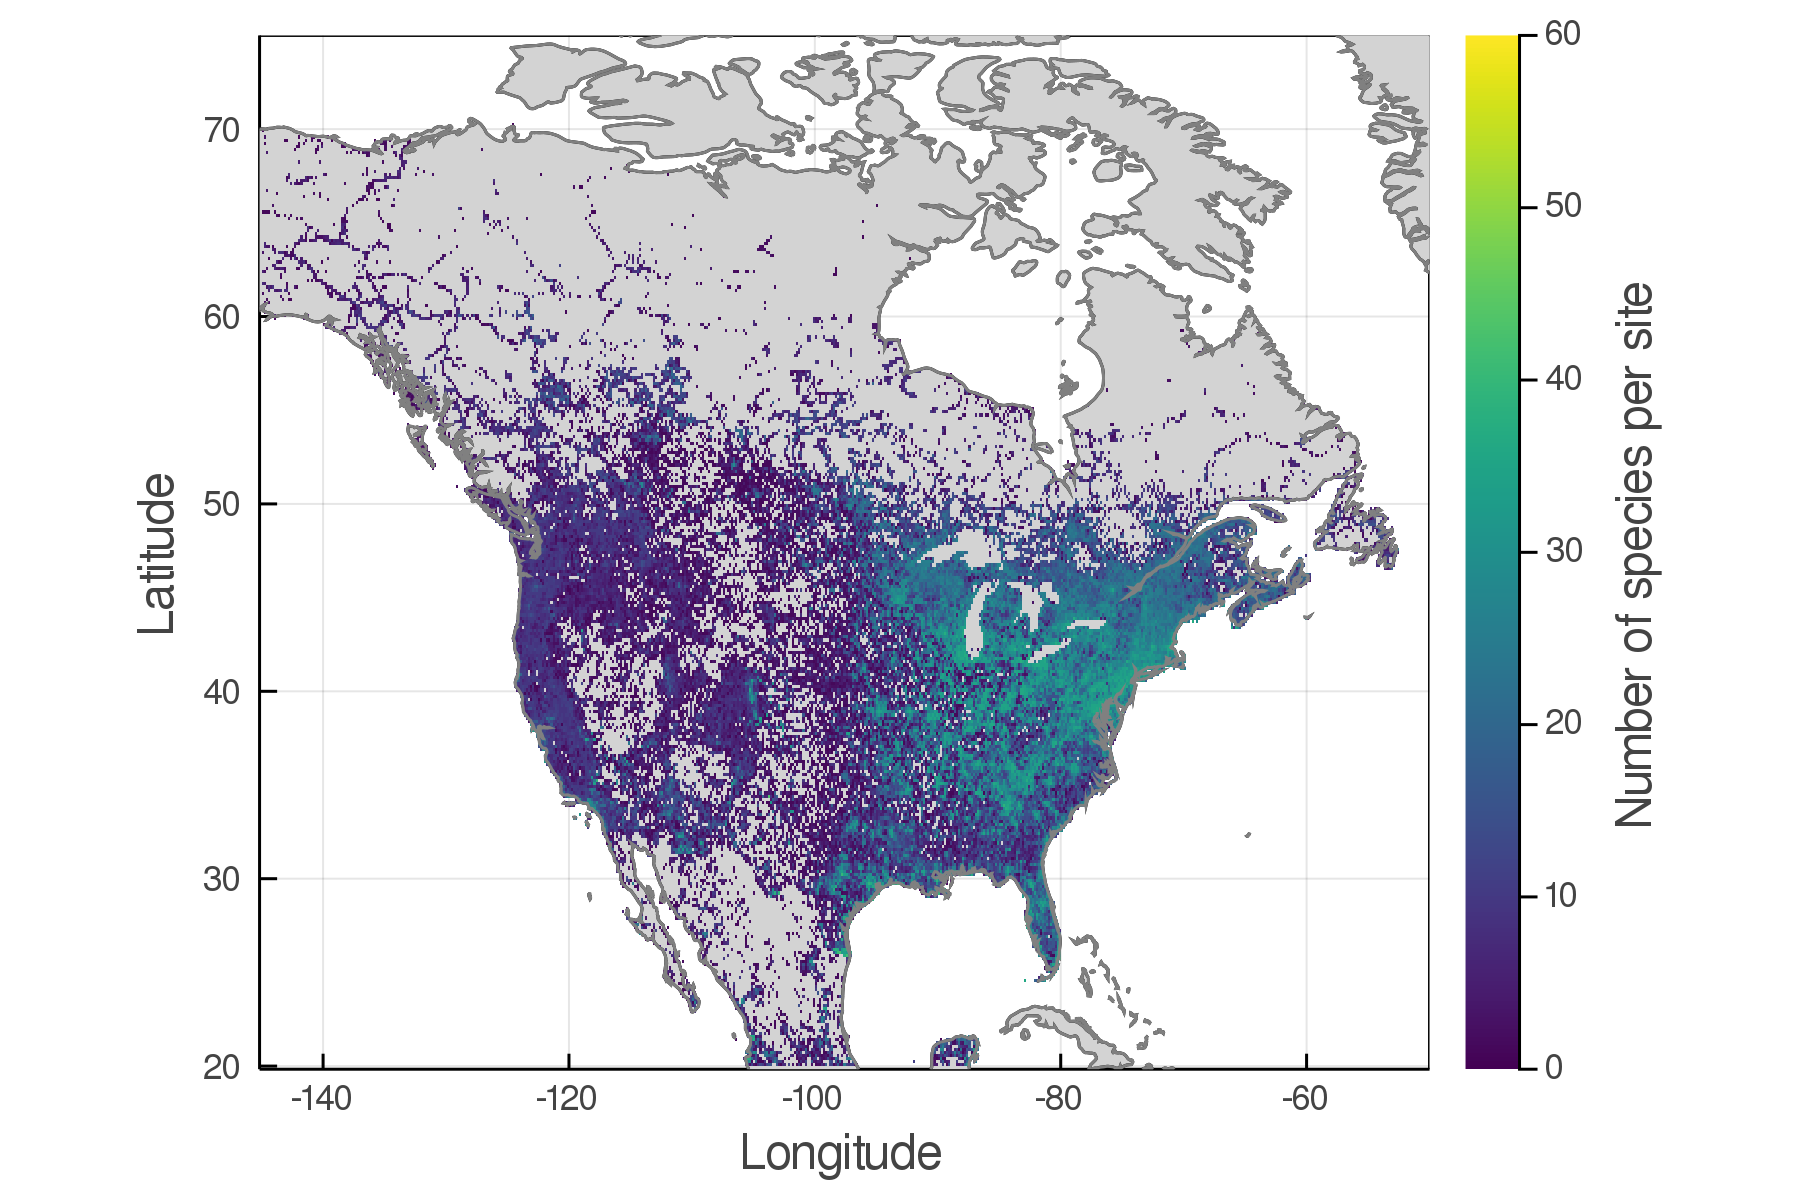
\includegraphics[scale=0.17]{fig/03_raw_richness.png}
    \caption{Species richness based on the raw occurrence data, defined as the number of species present per site}
  \end{figure}
\end{frame}

\begin{frame}
  \frametitle{Species richness - SDM without threshold}
  \begin{figure}
    \centering
    \hspace*{-0cm}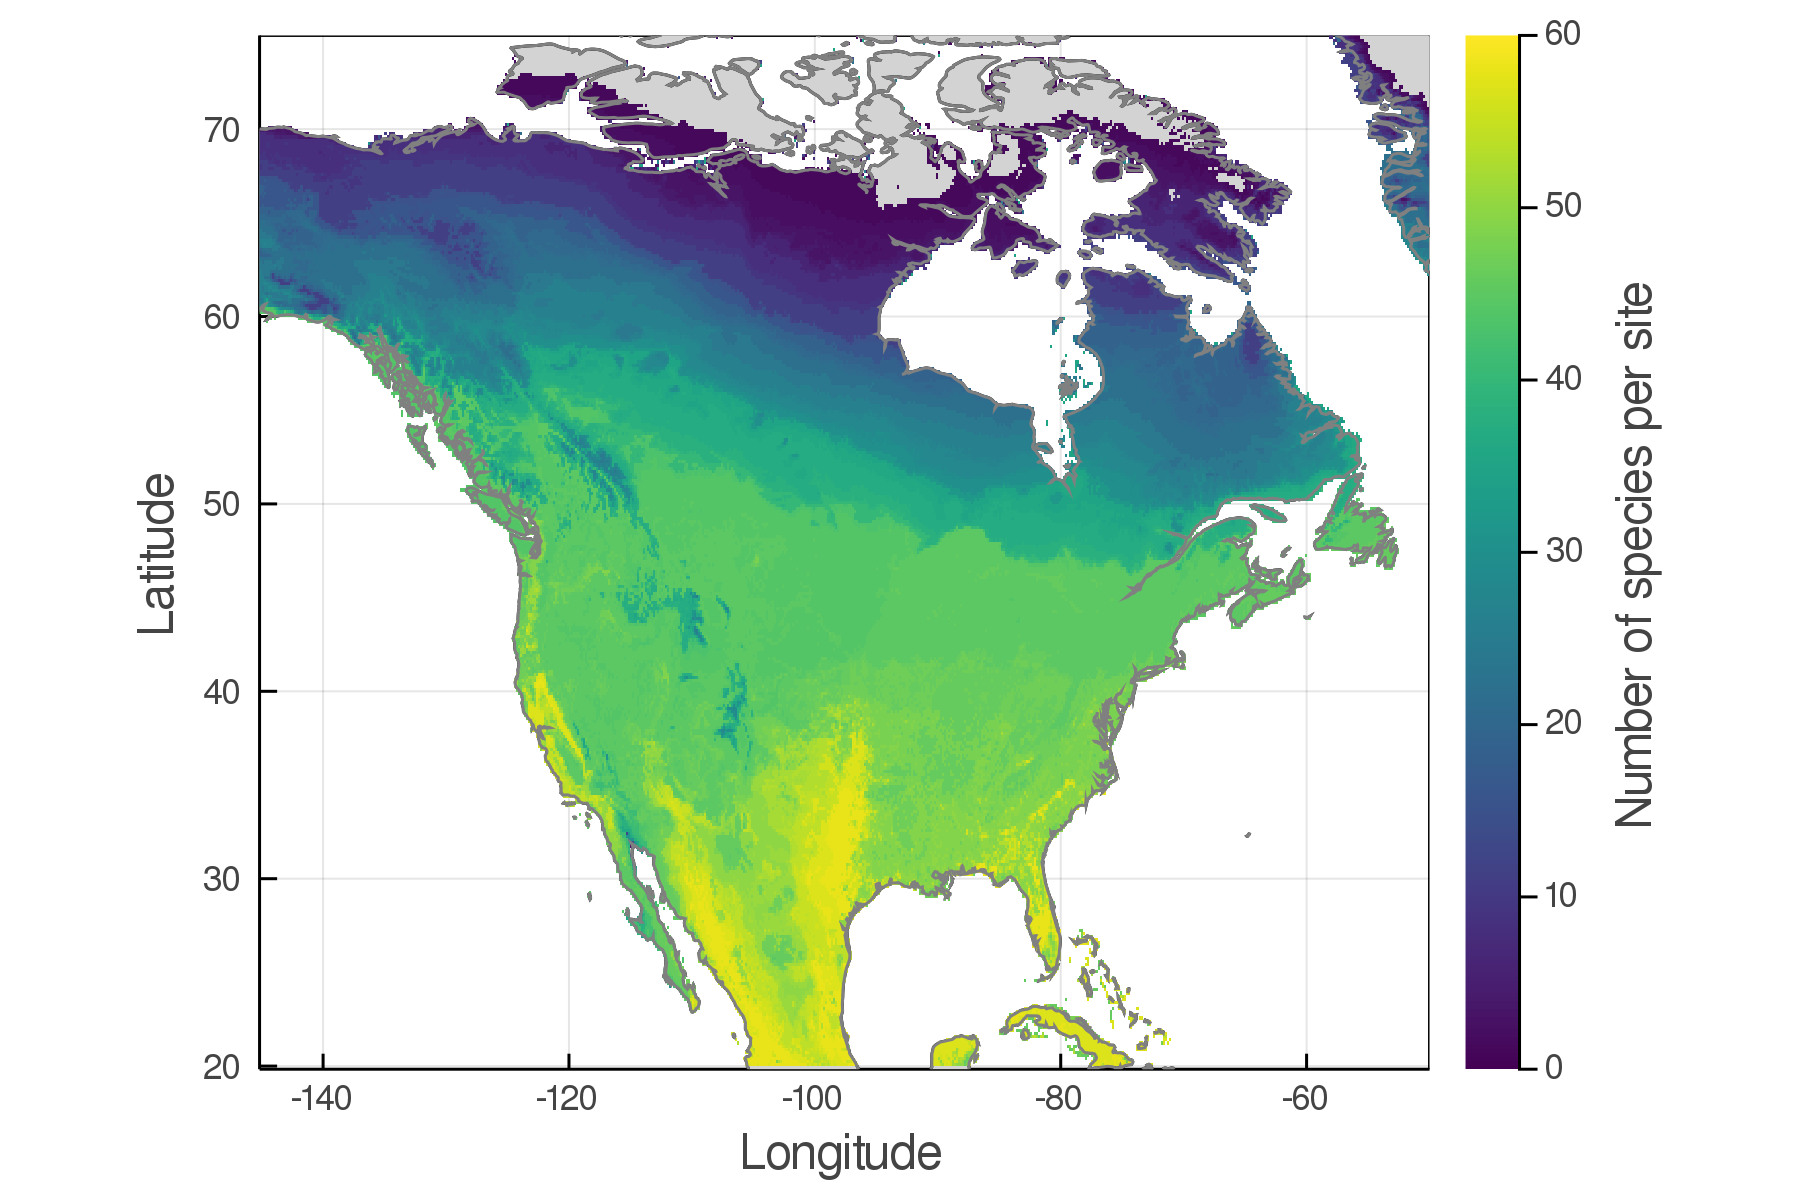
\includegraphics[scale=0.17]{fig/03_sdm_richness.png}
    \caption{Species richness based on the SDM predictions without threshold, and defined as the number of species present per site}
  \end{figure}
\end{frame}

\begin{frame}
  \frametitle{LCBD - Raw data (with Hellinger transformation)}
  \begin{figure}
    \centering
    \hspace*{-0cm}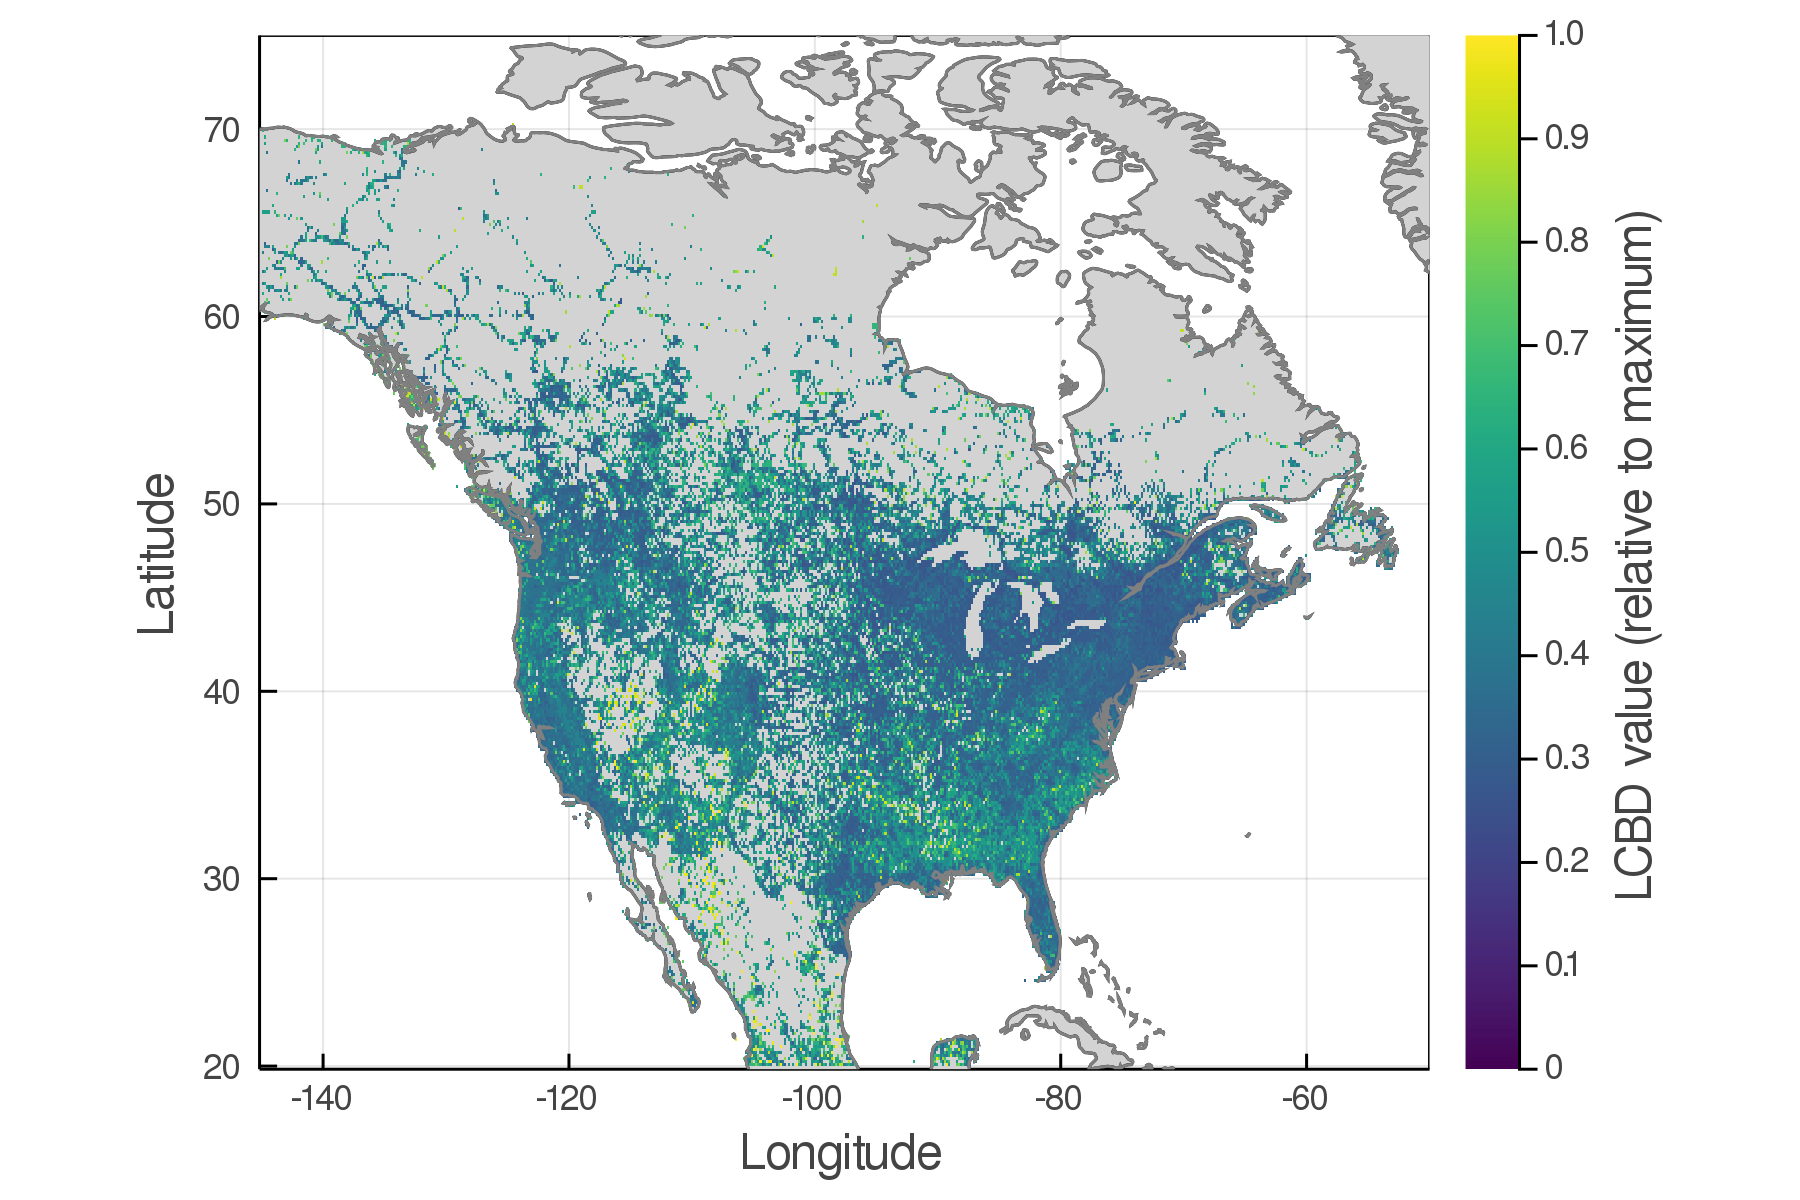
\includegraphics[scale=0.17]{fig/05_raw_lcbd-transf.png}
    \caption{LCBD values relative to maximum value based on the raw data after Hellinger transformation}
  \end{figure}
\end{frame}

\begin{frame}
  \frametitle{LCBD - SDM without threshold (no transformation)}
  \begin{figure}
    \centering
    \hspace*{-0cm}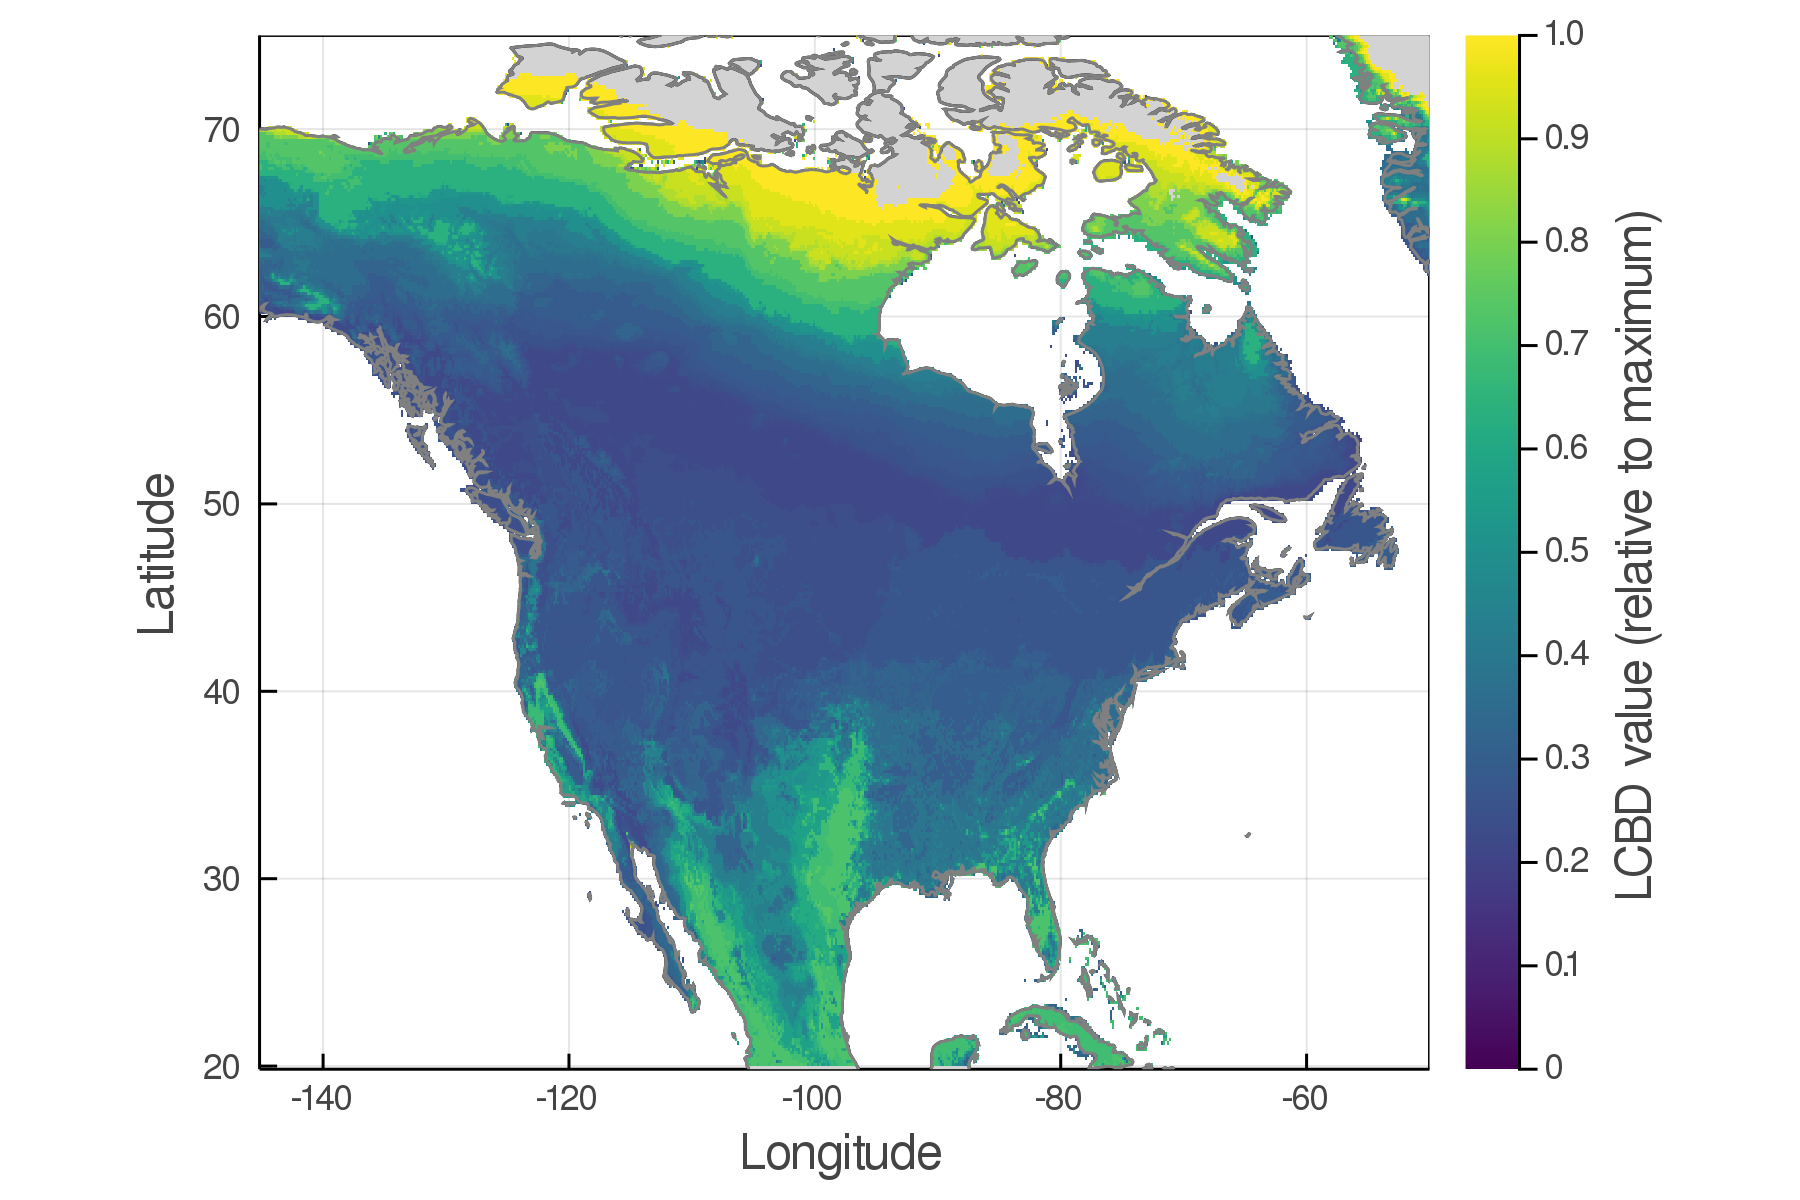
\includegraphics[scale=0.17]{fig/05_sdm_lcbd.png}
    \caption{LCBD values relation to maximum value based on the SDM predictions without threshold or transformation}
  \end{figure}
\end{frame}

\begin{frame}
  \frametitle{LCBD-richness relationship}
  \begin{figure}
    \centering
    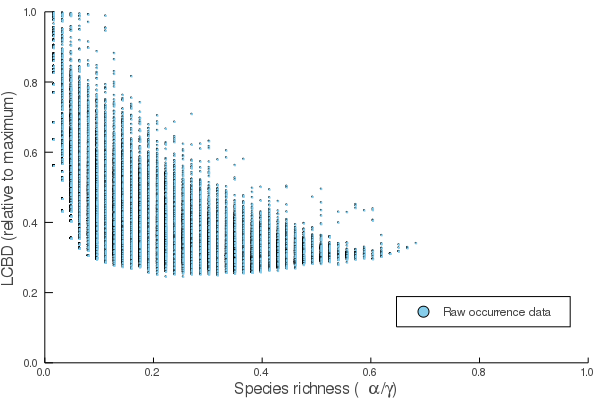
\includegraphics[scale=0.4]{fig/06_raw_relation.png}
    \caption{Relationship between the relative LCBD values and species richness, defined as the number of species ($\alpha$) divided by the total number of species ($\gamma$)}
  \end{figure}
\end{frame}

\begin{frame}
  \frametitle{LCBD-richness relationship}
  \begin{figure}
    \centering
    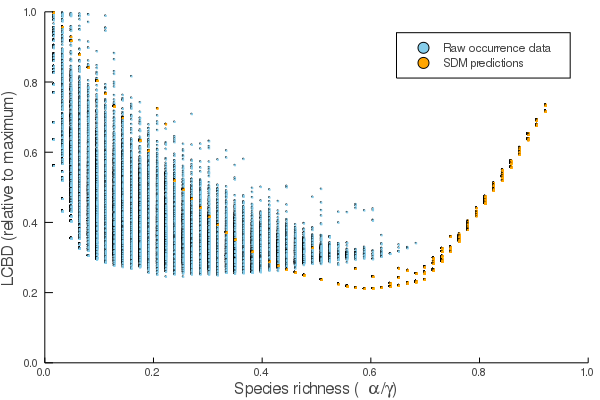
\includegraphics[scale=0.4]{fig/06_cmb_relation-oneplot.png}
    \caption{Relationship between the relative LCBD values and species richness, defined as the number of species ($\alpha$) divided by the total number of species ($\gamma$)}
  \end{figure}
\end{frame}

\begin{frame}
  \frametitle{Elements to discuss}
  \vfill
  Validating results
  \begin{itemize}
    \item Method for prediction error
    \item Data for evaluation
  \end{itemize}
  \vfill
  Improving SDM predictions
  \begin{itemize}
    \item Better modelling of presence-absence through environmental conditions
    \item Integrating other drivers of species distributions
  \end{itemize}
  \vfill
  Improving LCBD calculation \& understanding values
  \begin{itemize}
    \item Data transformation
    \item Relationship interpretation
  \end{itemize}
  \vfill
  Determining scale \& resolution to focus on
  \vfill
\end{frame}

\begin{frame}
  \frametitle{References}
  Johnston, A., W. M. Hochachka, M. E. Strimas-Mackey, V. Ruiz Gutierrez, O. J. Robinson, E. T. Miller, T. Auer, S. T. Kelling, and D. Fink. 2019. “Best Practices for Making Reliable Inferences from Citizen Science Data: Case Study Using eBird to Estimate Species Distributions.” bioRxiv, March, 574392. https://doi.org/10.1101/574392.
  \vfill
  Legendre, Pierre, and Miquel De Cáceres. 2013. “Beta Diversity as the Variance of Community Data: Dissimilarity Coefficients and Partitioning.” Ecology Letters 16 (8): 951–63. https://doi.org/10.1111/ele.12141.
  \vfill
  Poisot, Timothée, Cynthia Guéveneux‐Julien, Marie-Josée Fortin, Dominique Gravel, and Pierre Legendre. 2017. “Hosts, Parasites and Their Interactions Respond to Different Climatic Variables.” Global Ecology and Biogeography 26 (8): 942–51. https://doi.org/10.1111/geb.12602.
\end{frame}

\end{document}
